% mnras_template.tex 
%
% LaTeX template for creating an MNRAS paper
%
% v3.0 released 14 May 2015
% (version numbers match those of mnras.cls)
%
% Copyright (C) Royal Astronomical Society 2015
% Authors:
% Keith T. Smith (Royal Astronomical Society)

% Change log
%
% v3.0 May 2015
%    Renamed to match the new package name
%    Version number matches mnras.cls
%    A few minor tweaks to wording
% v1.0 September 2013
%    Beta testing only - never publicly released
%    First version: a simple (ish) template for creating an MNRAS paper

%%%%%%%%%%%%%%%%%%%%%%%%%%%%%%%%%%%%%%%%%%%%%%%%%%
% Basic setup. Most papers should leave these options alone.
\documentclass[fleqn,usenatbib]{mnras}

% MNRAS is set in Times font. If you don't have this installed (most LaTeX
% installations will be fine) or prefer the old Computer Modern fonts, comment
% out the following line
\usepackage{newtxtext,newtxmath}
% Depending on your LaTeX fonts installation, you might get better results with one of these:
%\usepackage{mathptmx}
%\usepackage{txfonts}

% Use vector fonts, so it zooms properly in on-screen viewing software
% Don't change these lines unless you know what you are doing
\usepackage[T1]{fontenc}

% Allow "Thomas van Noord" and "Simon de Laguarde" and alike to be sorted by "N" and "L" etc. in the bibliography.
% Write the name in the bibliography as "\VAN{Noord}{Van}{van} Noord, Thomas"
\DeclareRobustCommand{\VAN}[3]{#2}
\let\VANthebibliography\thebibliography
\def\thebibliography{\DeclareRobustCommand{\VAN}[3]{##3}\VANthebibliography}


%%%%% AUTHORS - PLACE YOUR OWN PACKAGES HERE %%%%%

% Only include extra packages if you really need them. Common packages are:
\usepackage{graphicx}	% Including figure files
\usepackage{amsmath}	% Advanced maths commands
\usepackage{amssymb}	% Extra maths symbols
\usepackage{multirow}   % Awful multirow table interface that I hate
\usepackage{tikz,xcolor,hyperref} % For the orcid icons that Paul implemented

%%%%%%%%%%%%%%%%%%%%%%%%%%%%%%%%%%%%%%%%%%%%%%%%%%

%%%%% AUTHORS - PLACE YOUR OWN COMMANDS HERE %%%%%

% Ripped from Paul's XXL-GAMA paper, cheers!
\definecolor{lime}{HTML}{A6CE39}
% Defines the ORCiD icon that goes next to the author's names
\DeclareRobustCommand{\orcidicon}{%
	
\begin{tikzpicture}
	\draw[lime, fill=lime] (0,0) 
	circle [radius=0.16] 
	node[white] {{\fontfamily{qag}\selectfont \tiny ID}};
	\draw[white, fill=white] (-0.0625,0.095) 
	circle [radius=0.007];
	\end{tikzpicture}
	\hspace{-2mm}
}

% Sets up the shortened ORCiD commands (e.g. \orcidA) that cause the icon and link to be added next to an author's name
\foreach \x in {A, ..., Z}{%
	\expandafter\xdef\csname orcid\x\endcsname{\noexpand\href{https://orcid.org/\csname orcidauthor\x\endcsname}{\noexpand\orcidicon}}
}

% Define the ORCID iD command for each author separately. 
% Turner
\newcommand{\orcidauthorA}{0000-0001-9658-1396}
% Giles
\newcommand{\orcidauthorB}{0000-0003-4937-8453}
% Romer
\newcommand{\orcidauthorC}{0000-0002-9328-879X}
% Wilkinson
\newcommand{\orcidauthorD}{0000-0002-3908-7313}
% Viana
\newcommand{\orcidauthorE}{0000-0003-1572-8531}
% Stott
\newcommand{\orcidauthorF}{0000-0002-1679-9983}
% Upsdell
\newcommand{\orcidauthorG}{0000-0003-0628-7201}
% Mann
\newcommand{\orcidauthorH}{0000-0002-0194-325X}
% Sahlen
\newcommand{\orcidauthorI}{0000-0003-0973-4804}
% Hilton
\newcommand{\orcidauthorJ}{0000-0002-8490-8117}


%%%%%%%%%%%%%%%%%%%%%%%%%%%%%%%%%%%%%%%%%%%%%%%%%%

%%%%%%%%%%%%%%%%%%% TITLE PAGE %%%%%%%%%%%%%%%%%%%

% Title of the paper, and the short title which is used in the headers.
% Keep the title short and informative.
% \title[XCS: Demonstrating the fidelity of eFEDS data products when applied to clusters of galaxies]{The XMM Cluster Survey: Demonstrating the fidelity of eFEDS data products when applied to clusters of galaxies}
\title[XCS: Demonstrating the fidelity of eFEDS data products when applied to clusters of galaxies]{The XMM Cluster Survey: An independent demonstration of the fidelity of the eFEDS galaxy cluster data products and implications for future studies}

\author[D. J. Turner et al.]
{D. J. Turner$^{1}$\thanks{E-mail: david.turner@sussex.ac.uk (DJT)}\orcidA{},
P. A. Giles$^{1}$\orcidB{},
A. K. Romer$^{1}$\orcidC{},
R. Wilkinson$^{1}$\orcidD{},
E. W. Upsdell$^{1}$\orcidG{},
S. Bhargava$^{2}$,
\newauthor
C. A. Collins$^{3}$,
M. Hilton$^{4,5}$\orcidJ{},
R. G. Mann$^{6}$\orcidH{},
M. Sahl\'en$^{7}$\orcidI{},
J. P. Stott$^{8}$\orcidF{},
P. T. P. Viana$^{9,10}$\orcidE{}
\\
% List of institutions
$^{1}$Department of Physics and Astronomy, University of Sussex, Brighton, BN1 9QH, UK\\
$^{2}$Département d’Astrophysique, CEA Paris-Saclay, 91190 Gif-sur-Yvette, France\\
$^{3}$Astrophysics Research Institute, Liverpool John Moores University, Liverpool Science Park, 146 Brownlow Hill, Liverpool L3 5RF, UK \\
$^{4}$Astrophysics Research Centre, University of KwaZulu-Natal, Westville Campus, Durban 4041, SA \\
$^{5}$School of Mathematics, Statistics, and Computer Science, University of KwaZulu-Natal, Westville Campus, Durban 4041, SA \\
$^{6}$Institute for Astronomy, University of Edinburgh, Royal Observatory, Blackford Hill, Edinburgh EH9 3HJ, UK \\
$^{7}$Department of Physics and Astronomy, Uppsala University, Box 516, SE- 751 20 Uppsala, Sweden\\
$^{8}$Department of Physics, Lancaster University, Lancaster LA1 4YB, UK \\
$^{9}$Instituto de Astrof\'isica e Ci\^{e}ncias do Espa\c co, Universidade do Porto, CAUP, Rua das Estrelas, 4150-762 Porto, Portugal \\
$^{10}$Departamento de F\'isica e Astronomia, Faculdade de Ci\^{e}ncias, Universidade do Porto, Rua do Campo Alegre, 687, 4169-007 Porto, Portugal \\
}

% These dates will be filled out by the publisher
\date{Accepted XXX. Received YYY; in original form ZZZ}

% Enter the current year, for the copyright statements etc.
\pubyear{2021}

% Don't change these lines
\begin{document}
\label{firstpage}
\pagerange{\pageref{firstpage}--\pageref{lastpage}}
\maketitle

% Abstract of the paper
\begin{abstract}
We present the first comparison between properties of clusters of galaxies measured by the eROSITA Final Equatorial-Depth Survey (eFEDS) and the XMM-Newton X-ray telescope. We have compared, in an ensemble fashion, properties from the eFEDS X-ray catalogue (542 candidates) with those from the Ultimate {\bf X}MM e{\bf X}traga{\bf L}actic (or XXL) survey project (100 clusters). We find the distributions of redshift and $T_{\rm X}$ to be broadly similar between the two surveys, with a larger proportion of clusters above 4keV in the XXL-100-GC sample. However, the fractional $\Delta T_{\rm X}$ values are significantly larger in eFEDS compared to XXL.
We construct a sample of 62 eFEDS X-ray cluster candidates that fall on an XMM observation, and inspect XMM, eROSITA, and SDSS images to remove candidates that should not be analysed. The final sample consists of 36 clusters, and we measure ${\sim}$24\% and ${\sim}$3\% contamination in the eFEDS X-ray and optically confirmed samples.
We then make direct comparisons of properties measured by eFEDS and by XMM for individual clusters using tools developed for the XMM Cluster Survey (XCS). Of our sample, 8 clusters have a $T_{\rm X}$ measured by both eROSITA and XMM, and we find and quantify an offset between the two telescopes. We compare 29 X-ray luminosities ($L_{\rm X}$) measured by eFEDS and XCS and find them to be in excellent agreement.  We also construct $L_{\rm X}$ - $T_{\rm X}$ scaling relations based on eFEDS and XCS measurements, which are in tension. The tension is decreased when we measure a third scaling relation with calibrated XCS temperatures, but they are still not wholly consistent.

% An understanding of how measurements from the two telescopes differ is essential for the pursuit of joint analyses and direct comparisons, including those requiring scaling relations.
% This does not necessarily imply that there is something wrong with the eROSITA calibration: a similar
% This is very encouraging for future eROSITA based cosmological studies as their analyses will largely be based on luminosity scaling relations.
\end{abstract}

% Select between one and six entries from the list of approved keywords.
% Don't make up new ones.
\begin{keywords}
keyword1 -- keyword2 -- keyword3
\end{keywords}

%%%%%%%%%%%%%%%%%%%%%%%%%%%%%%%%%%%%%%%%%%%%%%%%%%

%%%%%%%%%%%%%%%%% BODY OF PAPER %%%%%%%%%%%%%%%%%%

\section{Introduction}
X-ray observations of clusters of galaxies provide insights into various aspects of astrophysics  \cite[e.g.,][]{,hitomi16turb,bhargava20,sanders21} and cosmology \cite[e.g.,][]{, vikhlinincosmo, otherxraycosmo}.
Clusters are among the largest gravitationally bound structures in the Universe and consist of a dark matter halo, the intra-cluster medium, and the component galaxies. The intra-cluster medium (ICM) is a high-temperature, low-density, plasma that emits strongly in the X-ray band, with both continuum and emission line components.

%, and we can extract information about its density, temperature, and composition through observations with X-ray telescopes.

\begin{figure*}
    \centering
    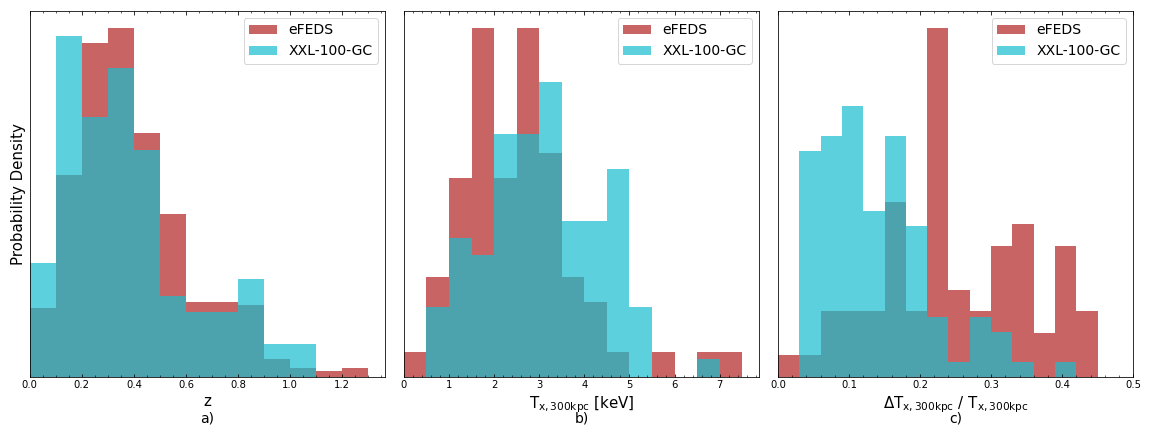
\includegraphics[width=1.0\textwidth]{images/efeds_xxl_z+t+t_frac.png}
    \caption[]{Redshift, temperature, and fractional temperature error distributions of the eFEDS and XXL-100-GC samples. Both sample's redshifts come from a variety of sources, and temperatures are measured within 300kpc apertures centered on clusters. Redshift distribution is of the whole eFEDS sample. There are no clusters in common between the two samples.} 
    \label{fig:xxlefeds}
\end{figure*}

%KR: not sure of the relevance of this paragraph
%It is also possible to derive the mass of a galaxy cluster from its X-ray emission, either directly through the assumption of hydrostatic equilibrium and the analysis of temperature and density radial profiles \citep[e.g.,][]{vikhlinin06,martino14,giles17}, or through the use of a scaling relation that takes us from an easier to measure quantity (such as a mean X-ray temperature/luminosity, or an optical richness) to an inferred mass \citep[e.g.,][]{efedsmor,xxlmt,arnaudmt}. Due to the difficulty of directly measuring galaxy cluster masses (using any method), these mass-observable relations (MORs) are essential for the derivation of cosmological parameters from galaxy cluster samples \citep[e.g.][]{desy1clusters}.

The eROSITA instrument mounted on the joint Russian-German Spectrum-Roentgen-Gamma (SRG) mission will contribute significantly to X-ray cluster astrophysics and cosmology. It's large field of view (${\sim}$1~deg), sensitivity (comparable to {\em XMM}), and energy resolution (also comparable to {\em XMM}) combine to make it a revolutionary new instrument. The final eROSITA All-Sky Survey (eRASS) is predicted to detect approximately 100,000 galaxy clusters above a mass of $5\times10^{13}$h$^{-1}$M$_{\odot}$. All of these clusters will be accompanied by an X-ray luminosity ($L_{\rm X}$) measurement, and roughly 20\% \citep[][]{efedsclustercat} of the observations will yield an X-ray temperature ($T_{\rm X}$) measurement. However, except for a handful of the highest flux clusters, it will not be  possible to measure masses, via the hydrostatic technique, directly from eRASS data. Therefore, in order to maximise the scientific yield of the survey, it will be necessary to supplement the eRASS cluster catalogue with mass measurements from the current generation of X-ray telescopes (i.e. {\em XMM}, {\em Chandra}). {\em eROSITA} will be used for pointed observations after the all sky survey is complete, as \cite{pointysanders} did during the commisioning phase.
% detail not needed: with more than 50 soft band (0.5-2.0keV) counts up to $\rm{z}\sim1$ \citep{erass_numclusters}.
The aim of this paper is to explore potential synergies between eRASS cluster catalogues and the data in the {\em XMM}-Newton public archives, calibration considerations required for such analyses, and to demonstrate the fidelity of eFEDS measurements. We wish to ascertain the level of contamination in the eFEDS cluster catalogue, verify the accuracy of $L_{\rm{X}}$ and $T_{\rm{X}}$ measurements, and compare the central coordinates of the detected clusters to those measured by the {\em XMM} Cluster Survey \citep[XCS, ][]{xcsfoundation}. As eFEDS is the same depth as the final eRASS, the accuracy of these measurements have implications for cosmological studies based on eRASS cluster detection (using weak lensing masses and X-ray luminosities for the mass observable relation). They will also impact studies based on optical or near-infrared detection (as luminosities can be used to explore scatter in the mass observable relations), and astrophysical studies of clusters luminosity-temperature relations to study the evolution of the intra-cluster medium. There is a known difference between the galaxy cluster temperatures measured by {\em XMM} and {\em Chandra} \citep[][]{xmmchandracal}. An understanding of whether there is a similar difference in {\em eROSITA} and {\em XMM} temperatures will be necessary before any joint analyses with data from the two telescopes is undertaken, and before scaling relations from one telescope can be safely used by another. For this we will make use of the recent release of the eROSITA Final Equatorial-Depth Survey \citep[eFEDS,][]{efedscat}. The eFEDS field covers approximately 140 square degrees of the equatorial ($-2.5^{\circ}<\delta<6.0^{\circ}$) sky. It intersects with several optical/near-IR photometry and/or spectroscopic surveys, including the Hyper Suprime-Cam Subaru Strategic Program \citep[HSC SSP, ][]{hscsurvey}, the Galaxy and Mass Assembly survey \citep[GAMA, ][]{gamasurvey}, and the Sloan Digital Sky Survey \citep[SDSS, ][]{sdss}.  Comparisons will be made to XCS measurements, as well as the XXL-100-GC catalogue \citep[][]{xxlgc100} to provide an indirect comparison to a similar X-ray survey.

% something for discussion, not intro: Interestingly, studies of clusters observed with both {\em XMM} and {\em Chandra}, has shown a significant difference between values of T$_{\rm{x}}$ measured for the same galaxy cluster.  This has led to functions to calibrate this observed temperature difference \citep[][]{xmmchandracal}, and any analysis which uses both XMM and Chandra temperatures typically accounts for this \citep[][]{farahixmmchandra,mikgasxmmchandra}.  
%not needed: The aim of this paper is to measure potential temperature differences between clusters detected in eFEDS, and those measure by {\em XMM}.

In \S\ref{sec:efedsproperties} we explore the general properties of the eFEDS cluster catalogue and provide comparisons to a catalogue with similar properties. In \S\ref{sec:efedsxmm} we construct a cluster sample from eFEDS with corresponding observations from {\em XMM} and match to sources detected in the {\em XMM} Cluster Survey. \S\ref{sec:meascomp} compares temperatures and luminosities measured by eFEDS and {\em XMM}. Finally, in \S\ref{sec:discussion} and \S\ref{sec:summary}, we generate luminosity-temperature relations, discuss implications of our findings and how it can be improved, and compare eFEDS and XCS central positions, then provide a final summary.

Throughout this work we use a concordance $\Lambda$CDM cosmology where $\Omega_{\rm{M}}$=0.3, $\Omega_{\Lambda}$=0.7, and $\rm{H}_{0}$=70 km s$^{-1}$ Mpc$^{-1}$, consistent with the original eFEDS cluster analysis (and other XCS works).

\section{Comparison of the \lowercase{e}FEDS Optically Confirmed and XXL-100-GC catalogues}
\label{sec:efedsproperties}

%KR: should this paragraph be in the into?
The eFEDS cluster catalogue \citep{efedsclustercat} contains 542 candidates, 477 of which are optically confirmed \citep{efedsclusteropticalcat}. All 542 X-ray candidates are accompanied by $z$ values, and soft-band $L_{\rm X}$ values have been measured for 91\% of the X-ray sample. Average $T_{\rm X}$ values were obtained for 69 (300kpc) and 95 (500kpc) of the candidates, with the apertures centered on the eFEDS. Accounting for overlap, $T_{\rm X}$ values have been measured for 102 candidates, all of which are in the optically confirmed sample (i.e. 21\% of 477).

\begin{figure*}
    \centering
    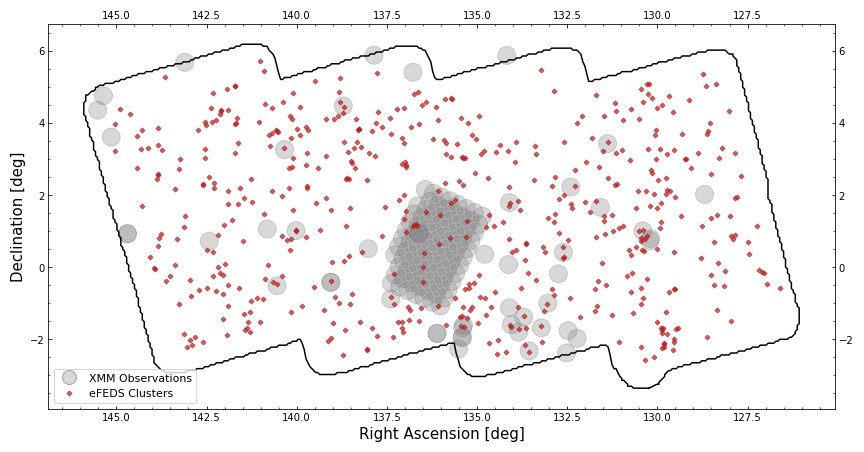
\includegraphics[width=1.0\textwidth]{images/outline_withborder.png}
    \caption[]{Footprint of eFEDS, given by the black solid line. Cluster candidates present in the eFEDS X-ray catalogue are highlighted by red diamonds. The grey circles highlight {\em XMM} observations, with a radius of 15\arcmin (the approximate radius of the {\em XMM} FoV).}
    \label{fig:efedsxcsclusters}
\end{figure*}

The XXL survey \citep{xxlfoundation} covers ${\sim}50$~deg$^2$ of the sky (over two separate regions), the largest contiguous area covered by {\em XMM}, and are made up of 542 separate {\em XMM} observations with on-axis exposure times ranging from 10-20ks.  The contiguous nature of XXL makes it an ideal point of comparison to eFEDS.  Note however that the XXL and eFEDS surveys were taken in different parts of the sky, providing no clusters in common, therefore, a direct comparison of individual clusters is not possible.  Comparisons are limited here to ensemble distributions of the cluster samples.  We made use of the XXL-100-GC sample \citep{xxlgc100}, containing the 100 brightest galaxy clusters observed in XXL, and the 477 optically confirmed sample from eFEDS.  The flux limits of the eFEDS and XXL-100-GC cluster samples are also similar; ${\sim}10^{-14}\:\rm{erg}\:\rm{s}^{-1}\:\rm{cm}^{-2}$ for the whole eFEDS cluster candidate catalogue, $4.9\times10^{-14}\:\rm{erg}\:\rm{s}^{-1}\:\rm{cm}^{-2}$ for the eFEDS candidates with a measured temperature value in a 500kpc aperture, and $3\times10^{-14}\:\rm{erg}\:\rm{s}^{-1}\:\rm{cm}^{-2}$ for XXL-100-GC. These flux limits are calculated using slightly different methods, but even so their similarity justifies a comparison between these two samples.

%Due to the contiguous and uniform nature of the eFEDS observations, it is natural to compare the overall sample properties to the XXL-100-GC sample \citep{xxlgc100}, which contains the 100 brightest galaxy clusters observed in the XXL \citep{xxlfoundation} fields. Combined, these fields cover ${\sim}50$ deg$^2$, and are made up of 542 separate {\em XMM} observations with on-axis exposure times ranging from 10-20ks. The flux limits of the eFEDS and XXL-100-GC cluster samples are also similar; ${\sim}10^{-14}\:\rm{erg}\:\rm{s}^{-1}\:\rm{cm}^{-2}$ for the whole eFEDS cluster candidate catalogue, $4.9\times10^{-14}\:\rm{erg}\:\rm{s}^{-1}\:\rm{cm}^{-2}$ for the eFEDS candidates with a measured temperature value in a 500kpc aperture, and $3\times10^{-14}\:\rm{erg}\:\rm{s}^{-1}\:\rm{cm}^{-2}$ for XXL-100-GC. These flux limits are calculated using slightly different methods, but even so their similarity justifies a comparison between these two samples.

Figure~\ref{fig:xxlefeds}a shows the redshift distributions of the clusters in the two samples (the eFEDS and XXL-100-GC distributions are shown in red and cyan respectively) to be very similar overall, but that XXL detects a higher proportion of clusters at low redshifts, and eFEDS has higher redshift candidates.  Next, we compare the respective temperature distributions.  Temperatures estimated for XXL clusters were measured within a 300kpc aperture \citep{xxllt}, as done for eFEDS clusters, making a direct comparison of the distributions valid. Figure~\ref{fig:xxlefeds}b plots the temperature distributions of the two samples, with the XXL temperature distribution containing a significantly higher proportion of temperatures above ${\sim}4\:\rm{keV}$. It is noted in \cite{efedsclustercat} that the ability to measure temperatures for hot clusters at $>$5~keV is limited due to the reduced sensitivity of eFEDS at energies $>$3 keV, this is a plausible reason of the increased number of higher temperature clusters in XXL compared to eFEDS ({\em eROSITA}'s effective area is ${\sim}$150~$\rm{cm}^2$ at 5~keV, compared to ${\sim}$900~$\rm{cm}^2$ for EPIC-PN). Furthermore, the temperature distribution could also be influenced by the selection functions of the two surveys, differing measurement methodology, or a systematic difference in temperatures measured by the {\em eROSITA} and {\em XMM} telescopes. Such a difference has been found between {\em XMM} and {\em Chandra}, and was recently calibrated by \cite{xmmchandracal}.

Finally we compare how well temperatures from the two samples are constrained, by comparing temperature uncertainties as a fraction of the absolute temperature value.  The temperature constraining power of XXL is shown to be greater than that of eFEDS in Figure~\ref{fig:xxlefeds}c, with the mean percentage uncertainties for XXL and eFEDS being 14\% and 25\% respectively. This fits with previous work by \cite{xcsmethod} that demonstrates ${\sim}2000$ background-subtracted soft-band (0.5-2.0keV) counts are required to achieve a fractional temperature uncertainty of ${\sim}0.1$. This would give the longer exposures of XXL an advantage over the eFEDS field (especially in the {\em XMM}-LSS fields which covers ${\sim}$11 deg$^{2}$ in the XXL-N field). XXL was a ground breaking survey, and maintains several key advantages in terms of temperature constraining power, but with the release of eFEDS it is no longer uniquely powerful.

\section{{\em XMM} counterparts to \lowercase{e}FEDS clusters}
\label{sec:efedsxmm}

\begin{table*}
\begin{center}
\caption[]{{Summary of the samples defined in this work. N$_{\rm{cl}}$ is the number of clusters, N$_{\rm{T}_{\rm{eFEDS, 3(5)00kpc}}}$ the number with eFEDS T$_{\rm{XCS, 3(5)00kpc}}$ values, and N$_{\rm{T}_{\rm{XCS, 3(5)00kpc}}}$ the number with XCS T$_{\rm{3(5)00kpc}}$ values.}\label{tab:samples}}
\vspace{1mm}
\begin{tabular}{l|lccccc}
\hline
\hline
Sample Name & Description & N$_{\rm{cl}}$ & N$_{\rm{T}_{\rm{eFEDS, 300kpc}}}$ & N$_{\rm{T}_{\rm{eFEDS, 500kpc}}}$ & N$_{\rm{T}_{\rm{XCS, 300kpc}}}$ & N$_{\rm{T}_{\rm{XCS, 500kpc}}}$\\
\hline
\hline
eFEDS & The full eFEDS cluster candidates catalogue & 542 & 69 & 95 & - & - \\
\hline
eFEDS-{\em XMM} & eFEDS cluster candidates that fall on an XMM observation & 62 & 8 & 11 & - & - \\
\hline
eFEDS-XCS & eFEDS-{\em XMM} candidates accepted after visual inspection & 36 & 6 & 8 & 23 & 29 \\
\hline
\end{tabular}
\end{center}
\end{table*}

In this section, we make use of archival {\em XMM} data that overlaps with the eFEDS footprint.  As such, we used the {\em XMM} Cluster Survey \citep[XCS,][]{xcsfoundation} cleaned data and source lists to: ({\em i}) determine which eFEDS cluster candidates fall on an {\em XMM} observation (Sect.~\ref{sec:eFEDS-XMM}); ({\em ii}) match the eFEDS candidates to an XCS extended source within these observations; ({\em iii}) verify that the candidates are clusters (utilising information from XCS, {\em eROSITA} and SDSS, Sect.~\ref{sec:efeds-varification}), providing examples of eFEDS candidates rejected from out analysis (Sect.~\ref{sec:examplerejects}); and ({\em iv}) understand the contamination fraction in the eFEDS sample (Sect.~\ref{sec:contamfrac}).

\begin{figure}
    \centering
    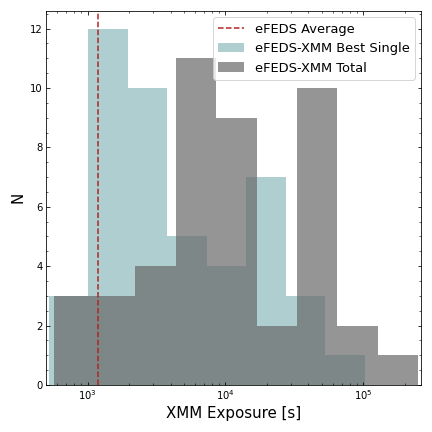
\includegraphics[width=0.95\columnwidth]{images/xmm_exposures.png}
    \caption[]{Distribution of exposure times for eFEDS-{\em XMM} cluster candidates, measured at the eFEDS coordinates. Exposures taken from 0.5-2.0keV exposure maps, corrected for flaring and vignetting. Dashed line indicates the average vignetting corrected exposure of the eFEDS field reported by \cite{efedsclustercat}.}
    \label{fig:xmmexposure}
\end{figure}

\subsection{\lower{e}FEDS Cluster Candidates in the {\em XMM} Footprint}
\label{sec:eFEDS-XMM}

Figure~\ref{fig:efedsxcsclusters} shows the outline of the eFEDS footprint with eFEDS X-ray cluster candidates \citep{efedsclustercat} indicated by red diamonds. {\em XMM} observations taken within the eFEDS footprint are given by grey shaded circles, with a radius of 15$^{\prime}$ (the approximate field-of-view of {\em XMM}). Given there are 143 {\em XMM} observations, covering a total of {\color{red} ***} deg$^{2}$ of the eFEDS footprint, Figure~\ref{fig:efedsxcsclusters} highlights the extraordinary field of view of {\em eROSITA} and its utility as a survey instrument when compared to {\em XMM}. 
%as well as showing us that the majority of eFEDS cluster candidates do not fall on an {\em XMM} observation.

We used {\em XMM}: Generate and Analyse \citep[\texttt{XGA}\footnote{\href{https://github.com/DavidT3/XGA}{{\em XMM}: Generate and Analyse GitHub}}][]{xgapaper}; a new, open-source, X-ray astronomy analysis module developed by XCS, to determine which eFEDS cluster candidates fall within the footprint of an {\em XMM} observation. The 542 eFEDS clusters given in \cite{efedsclustercat} were used (instead of the 477 optically confirmed clusters), allowing for the study of non-confirmed clusters with potentially deeper {\em XMM} data to understand the eFEDS selection.

An initial search is performed using the XCS archive of cleaned event lists for observations with an aimpoint that falls within 30\arcmin of a candidate (at the eFEDS coordinates). We then applied the requirement that 70\% of a 300kpc aperture (assuming the eFEDS redshift) falls on an {\em XMM} camera.  This search returned 62 eFEDS X-ray cluster candidates have been observed by {\em XMM}, and this sub-set is denoted the eFEDS-{\em XMM} sample.

% Near the centre of Figure~\ref{fig:efedsxcsclusters} we can see a significant collection of {\em XMM} observations, the Herschel-ATLAS contiguous field followups. The majority of the {\em XMM}-HATLAS observations are shallow, with requested exposures of ${\sim}$2.5ks. While this makes it relatively comparable to the depth of the eFEDS (and eRASS) fields, it unfortunately means that it is likely to be difficult to measure well constrained temperatures for many of the clusters in this field.

The distribution in Figure~\ref{fig:xmmexposure} demonstrates that the majority of eFEDS cluster candidates that fall on an XMM observation have a longer exposure time in {\em XMM} than the average 1.2ks vignetting-corrected exposure reported by \cite{efedsclustercat}. Though a direct exposure time comparison does not tell us everything about the relative usefulness of the {\em XMM} and {\em eROSITA} data (it is complicated by the relative effective area curves, as well as the different locations of the telescopes resulting in different levels of flaring and particle background), it does highlight that {\em XMM}-Newton observations (both new and archival) will continue to be important into the era of {\em eROSITA}, despite the impressive capabilities and field of view of the new telescope. 


\subsection{Verifying the eFEDS-{\em XMM} Cluster Candidates}
\label{sec:efeds-varification}

%Now that we have a sample of eFEDS cluster candidates that have also been observed by {\em XMM}, we need to verify that they are galaxy clusters, that the {\em XMM} data are of a high enough quality for us to analyse, and whether they have been detected by XCS. We do not necessarily expect that the entire eFEDS-{\em XMM} sample will have high enough quality data for us to confirm or deny an eFEDS candidate, or measure X-ray properties for them. 

%XCS is a serendipitous survey utilising the entire archive of {\em XMM} observations to locate X-ray sources, with a focus on detecting galaxy clusters. Source detection is performed using a custom version of WAVDETECT \citep{wavdetect} called the XCS Automated Pipeline Algorithm \citep[XAPA,][]{xcsmethod}. XAPA is run on merged EPIC (PN+MOS1+MOS2) images, generated using events within an energy range of 0.5-2.0keV. This energy range is similar, but not identical, to the energy band in which eFEDS performed their source detection (0.2–2.3keV). Sources detected within separate {\em XMM} observations are then combined into an XCS Master Source List (XCS-MSL). As of mid 2020 this contains 327205 objects, of which 39890 (12\%) are classified as extended, and 332315 (88\%) are classified as point sources. 

Using the 62 clusters in the eFEDS-{\em XMM} sample, we generate {\em eROSITA} and {\em XMM} images in order to assess the quality of the {\em XMM} observations, compare the observations of the {\em XMM} and {\em eROSITA} telescopes and visually confirm the presence of X-ray emission.  {\em XMM} is an ideal telescope with which to perform direct {\em eROSITA} image comparisons; the detector properties are very similar, but both the EPIC-PN and EPIC-MOS cameras have a slightly smaller PSF effect.  The \texttt{eSASS} \texttt{evtool} software was used to generate images of {\em XMM} fields (centered on the same coordinates), while using the same binning and image size to ensure a scaling of 4.35\arcsec per pixel; this allowed a valid side-by-side comparison. Images were created in the energy bands used for source detection by the respective surveys, corresponding to 0.5-2.0~keV and 0.2-2.3~keV for XCS and eFEDS respectively.  Next, we utilised the XCS Master Source List (XCS-MSL) to determine those eFEDS clusters that are detected on corresponding {\em XMM} observations (to aid in visual inspection of the eFEDS clusters).  Construction of the MSL is fully described in \cite{xcsgiles}, and is generated from source detection performed on {\em XMM} images using the XCS Automated Pipeline Algorithm \citep[XAPA,][]{xcsmethod}, a custom version of WAVDETECT \citep{wavdetect} developed within XCS.  Based upon this initial visual inspection, 9 eFEDS candidates were excluded from further analysis due to the corresponding poor {\em XMM} data quality (see Table~\ref{tab:xmmrejects} for details).    

The remaining candidates (53 eFEDS-{\em XMM} candidates, after the 9 excluded above) were then visually inspected to confirm that these candidates are indeed galaxy clusters.  We made use of the SDSS (overlapping with the majority of eFEDS) in order to visually confirm the X-ray emission is associated with a cluster.  \cite{simerass} predicted that the contamination of the X-ray cluster candidate catalogue would be ${\sim}$20\%, and an eFEDS analysis by \cite{efedsclusteropticalcat} found a value in agreement with that prediction, hence the need for this visual inspection step.  The overall contamination of eFEDS is discussed further in Section~\ref{sec:contamfrac}.  We found 16 candidates where the ICM was significantly contamination, or they are spurious detections in eFEDS (i.e., a cluster was not responsible for the X-ray emission).  These 16 clusters were subsequently rejected from the final sample.  Notes on these 16 candidates are given Section~\ref{sec:notes} and listed in Table~\ref{tab:rejects}, with a detailed discussion of noteworthy candidates given in Section~\ref{sec:examplerejects}.  The rejection of these 26 candidates resulted in a final sample of 36 cluster candidates, with this sub-set denoted the eFEDS-XCS sample. 

\subsubsection{Notes on rejected clusters}
\label{sec:notes}

Here we provide notes on the 16 clusters rejected in Section~\ref{sec:efeds-varification}:
\begin{itemize}
\item[] \noindent 1644 -- X-ray emission appears coincident with two interacting active galaxies (see Sect.~\ref{sec:examplerejects}).
\item[] \noindent 3334 -- No significant X-ray emission in eFEDS or XMM (see Sect.~\ref{sec:examplerejects}).
\item[] \noindent 8602 -- eFEDS candidate split into two detections by eFEDS (see Sect~\ref{sec:examplerejects}).
\item[] \noindent 1376 -- XMM data to shallow for confirmation.  There is a cluster there, but eFEDS coordinate is offset from the extended emission. 
\item[] \noindent 5909 -- eFEDS candidate detected as a point source in XCS.  There are no galaxies coincident with the X-ray emission in SDSS.
\item[] \noindent 8922 -- Spurious detection in the outskirts of a bright point source (see Sect.~\ref{sec:examplerejects}).
\item[] \noindent 16370 -- eFEDS candidate coincident with a collection of galaxies in SDSS.  However, X-ray emission contaminated by low redshift point source (see Sect.~\ref{sec:examplerejects}).
\item[] \noindent 9463 -- eFEDS candidate detected as two separate point sources in XCS using deeper {\em XMM} data.
\item[] \noindent 13484 -- No obvious extended X-ray emission in eFEDS or {\em XMM}.  There are no evidence of cluster galaxies in SDSS at the eFEDS measured redshift (z=0.317).
\item[] \noindent 13299 -- Spurious detection in the outskirts of the X-ray emission of a bright star.
\item[] \noindent 150 -- X-ray extended emission dominated by a massive elliptical galaxy(see Sect.~\ref{sec:examplerejects}).
\item[] \noindent 11754 -- Spurious detection in the outskirts of eFEDS 150.
\item[] \noindent 3133 -- SDSS indicates the presence of a group of galaxies, however, the eFEDS emission is likely dominated by the central massive elliptical galaxy.
\item[] \noindent 3008 -- SDSS indicates the presence of a group of galaxies, however, the eFEDS emission is likely dominated by the central massive elliptical galaxy.
\item[] \noindent 5702 -- Deeper {\em XMM} observation reveals the X-ray emission is coming from a blue object in SDSS (which appears to be an AGN), XCS detects this as a point source (see Sect.~\ref{sec:examplerejects}).
\item[] \noindent 6840 -- eFEDS candidate appears to be coincident with a blue source in SDSS (potentially an AGN).  XCS detects {\em XMM} emission as a point source, again, coincident with the SDSS source.
\end{itemize}

\subsubsection{Examples of contamination in the eFEDS X-ray cluster candidate catalogue}
\label{sec:examplerejects}

\begin{figure*}
    \centering
    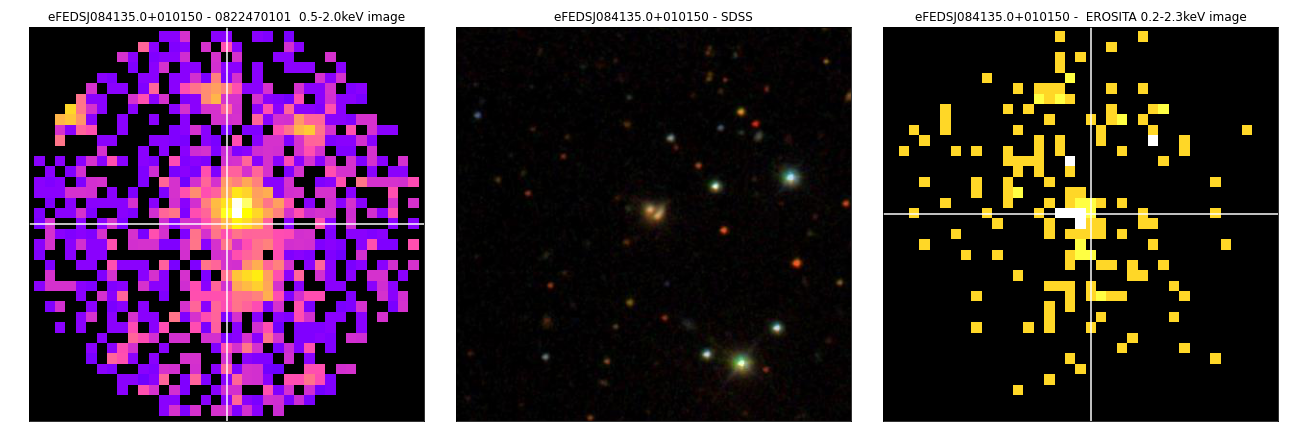
\includegraphics[width=1\textwidth]{images/interactingagn.png}
    \caption[]{eFEDS-{\em XMM} candidate (ID 1644) identified as a pair interacting galaxies with ongoing AGN activity (see Section~\ref{sec:examplerejects}). Left hand side is a combined PN+MOS1+MOS2 {\em XMM} image (ObsID 0822470101), centre is SDSS, right hand side is {\em eROSITA}.  Both {\em XMM} and {\em eROSITA} images are cutouts within a radius of 500~kpc (at the redshift provided by eFEDS).}
    \label{fig:pairagn}
\end{figure*}

Here we provide detailed descriptions on a number of the candidates rejected in Section~\ref{sec:efeds-varification}, along with images from {\em XMM}, {\em SDSS} and {\em eROSITA}.  The first example (eFEDS ID 1644) is shown in Figure~\ref{fig:pairagn}, which is a pair of interacting galaxies with bright AGN \citep[as discussed in][]{agnpair}.  The X-ray emission is detected as a point source in the {\em XMM} image (Fig~\ref{fig:pairagn}, left) by XCS, coincident with the pair of galaxies in SDSS (Fig~\ref{fig:pairagn}, middle).  Another nearby point source is clearly visible in the {\em XMM} image (again detected as a point source by XCS).  The shallower detected in eFEDS (Fig~~\ref{fig:pairagn}, right) has potentially blended these two sources leading to the detection of a single extended source by the eROSITA source finder.

In Figure~\ref{fig:brightoutskirts} we found that eFEDS (ID 8922) has spuriously identified a cluster candidate in the outskirts of a bright point source (a behaviour that is also seen in two other eFEDS-{\em XMM} candidates).  The point source is clearly detected in {\em XMM} (Fig~\ref{fig:brightoutskirts}, left) and coincident with a spiral galaxy with a central AGN in SDSS (Fig~\ref{fig:brightoutskirts}, middle).  The source is identified as an AGN in the Million Quasar catalog \citep{milliquas}.  The coordinates of the eFEDS candidate (given by the white cross-hairs) is clearly in the outskirts of the X-ray emission from the point source in eFEDS (Fig~\ref{fig:brightoutskirts}, right).  The smaller PSF of {\em XMM} shows little extended emission at these coordinates, and we conclude this is a spurious detection in eFEDS.

\begin{figure*}
    \centering
    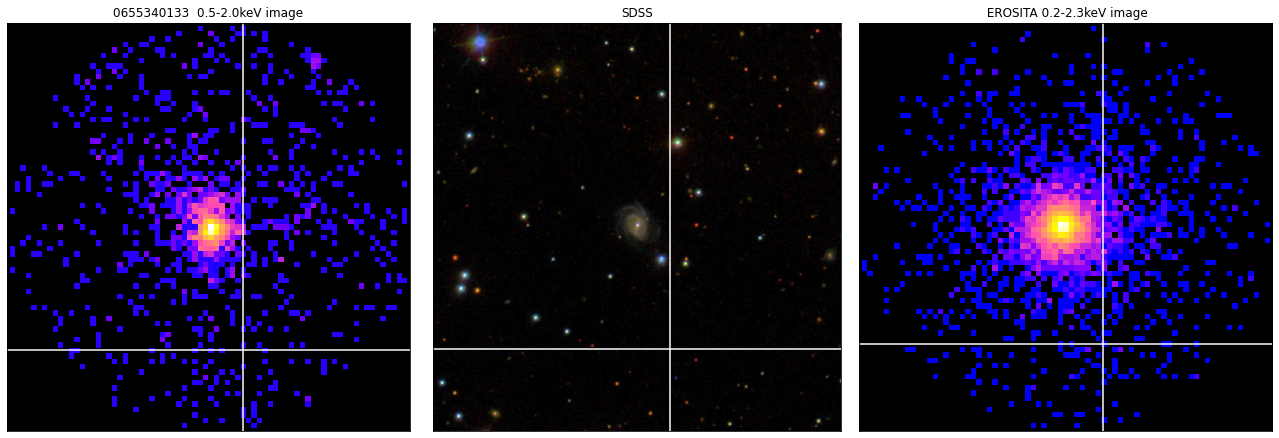
\includegraphics[width=1\textwidth]{images/outskirt_cands.png}
    \caption[]{Spurious eFEDS-{\em XMM} cluster candidate (ID 8922) found in the outskirts of a bright point source.  The X-ray emission is dominated by a low redshift AGN (see Section~\ref{sec:examplerejects}). Left hand side is {\em XMM}, middle is SDSS, and right is {\em eROSITA}.}
    \label{fig:brightoutskirts}
\end{figure*}

Another eFEDS-{\em XMM} candidate (ID 16370) is also present in Figure~\ref{fig:brightoutskirts}.  The eFEDS candidate is highlighted by the white circle.  While no obvious X-ray emission is present, the coordinates coincide with a collection of red galaxies in SDSS at a photo-z of z=0.44 (matching the eFEDS catalog).  Due to the proximity of the eFEDS candidate to the bright point source, we exclude this cluster from our analyses due to contamination of any X-ray emission from the cluster due to the foreground AGN.

\begin{figure}
    \centering
    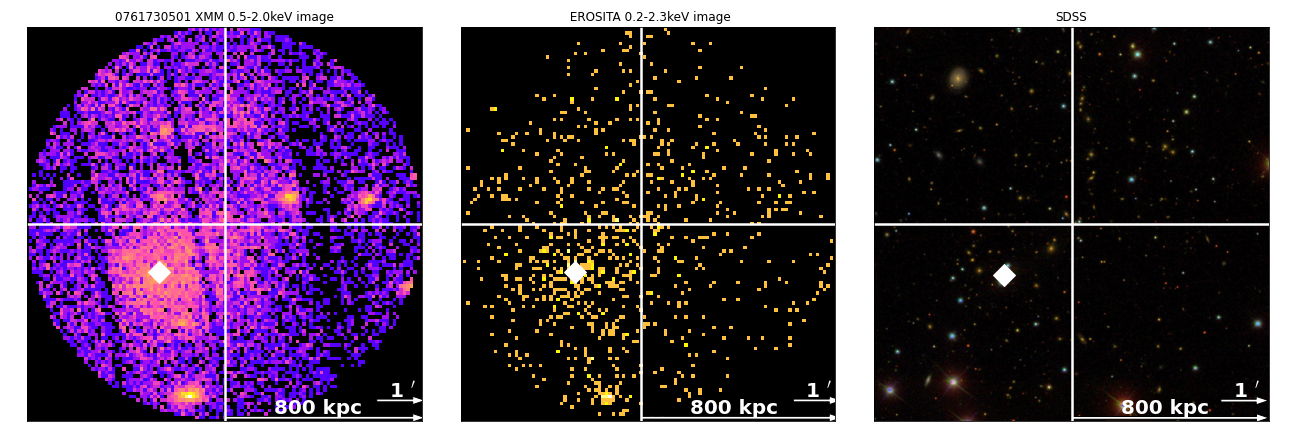
\includegraphics[width=1\columnwidth]{images/split_cluster.png}
    \caption[]{Example of an eFEDS cluster candidate, split into two sources by the eFEDS cluster finder. Cross-hairs indicate one candidate (eFEDS J085022.3+001607), and the diamond indicates the other (eFEDS J085027.9+001503). Left image is {\em XMM}, right is {\em eROSITA}.}
    \label{fig:splitcluster}
\end{figure}

During our visual inspection of the eFEDS-{\em XMM} candidates, we found one instance where the detection of a high signal-to-noise cluster candidate in eFEDS has been split into two separate entries in the X-ray cluster catalogue. Figure~\ref{fig:splitcluster} shows {\em XMM} and {\em eROSITA} images of the cluster, with the white cross-hair indicating the position of the first cluster fragment (eFEDS J085022.3+001607), and the white diamond the other fragment (eFEDS J085027.9+001503). The two eFEDS-XMM candidates have almost identical eFEDS redshifts (0.196 and 0.197 respectively), both have measured eFEDS luminosities, however, only eFEDS J085027.9+001503 has a temperature measurement. Unfortunately we are forced to exclude both candidates, even though the second is one of the few candidates that has an eFEDS temperature measurement and high quality {\em XMM} data; this is because we expect that part of the cluster will have been excluded in the eFEDS analysis, and as such the temperature and luminosity are invalid. 

\begin{figure*}
    \centering
    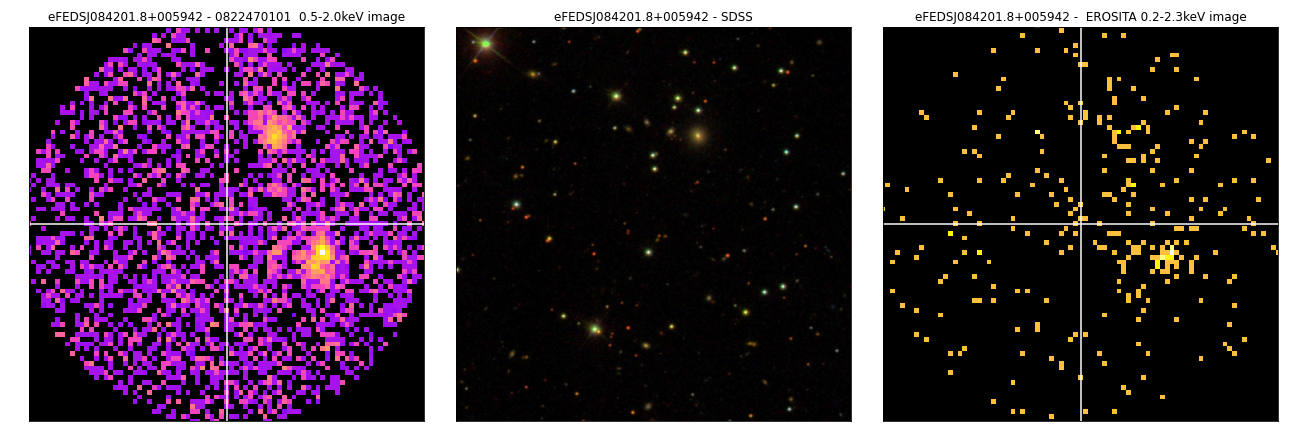
\includegraphics[width=1\textwidth]{images/blanklowz_sdss.png}
    \caption[]{An eFEDS-{\em XMM} cluster candidate (eFEDS J084201.8+005942) without an obvious corresponding source of emission. The cross-hair indicates the eFEDS position, with a 3\arcmin aperture. Left image is {\em XMM}, middle is SDSS, right is {\em eROSITA}.}
    \label{fig:blanksky}
\end{figure*}

{\bf We also observed cases where no X-ray source is present in {\em XMM} or {\em eROSITA} images. Figure~\ref{fig:blanksky} is an example where we cannot locate a source at the eFEDS coordinates (extended or otherwise) in the image taken by either X-ray telescope (with the {\em XMM} observation being deeper than eFEDS), and as such it is hard to know what the eFEDS source finder detected here. The redshift provided by the eFEDS cluster catalogue for this candidate (eFEDS J084201.8+005942) is very low (0.087).  Inspection using SDSS does not indicate any overdensity of galaxies at the eFEDS coordinates.  Therefore, the eFEDS detection remains somewhat of a mystery.} \textcolor{red}{\bf Swap this with discussion of 5702.  X-ray emission coming from AGN, present in Milliquas}  

\begin{figure*}
    \centering
    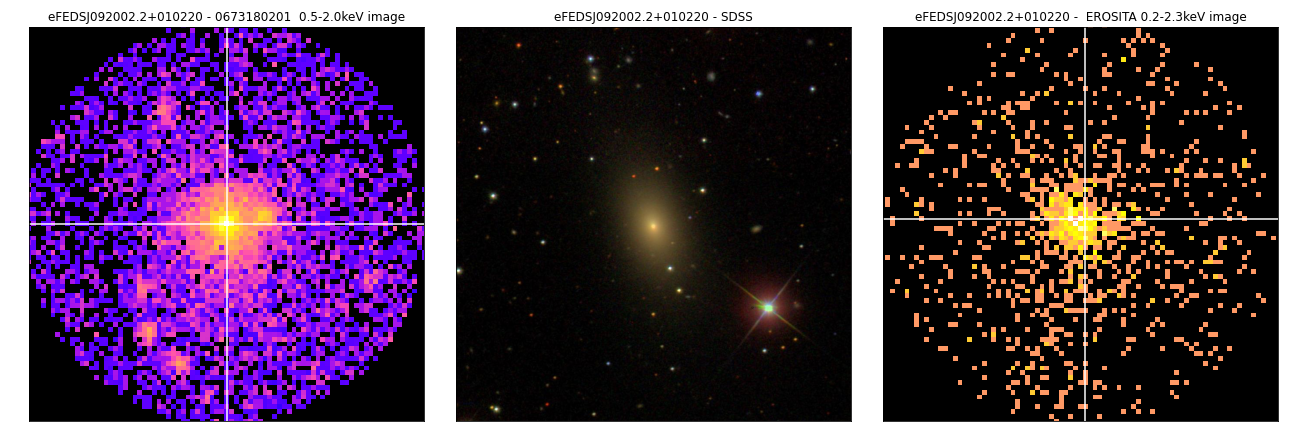
\includegraphics[width=1\textwidth]{images/elliptical_xray.png}
    \caption[]{An eFEDS-{\em XMM} cluster candidate (eFEDS J092002.2+010220) that appears to be a low-redshift, bright, X-ray emitting elliptical galaxy. Aperture applied to the X-ray data is centered on eFEDS coordinates, has a radius of 3\arcmin, and SDSS image is the same size. Left image is {\em XMM}, middle is SDSS, right is {\em eROSITA}.}
    \label{fig:ellipticalxray}
\end{figure*}

Finally, we encountered two cases where X-ray emission attributed to a galaxy cluster was significantly contaminated by an X-ray bright elliptical galaxy. We consider these sources (eFEDS J092002.2+010220 and eFEDS J092235.9-002443) to be low redshift groups.  Figure~\ref{fig:ellipticalxray} shows the {\em XMM} and {\em eROSITA} images related to the first of these candidates, with the addition of an SDSS image for further context. The extended X-ray emission appears to dominated by the galaxy, rather than any significant emission from an intra-group medium.

%\subsection{Constructing the \lower{e}FEDS-XCS cluster sample}

%Based upon visual inspection, we rejected 26 of the 62 candidates in the eFEDS-{\em XMM} sample (as discussed below) and are not included for further analysis.  Of these rejected candidates, 7 were rejected due to poor quality {\em XMM} data (see Table~\ref{tab:xmmrejects} for further information), hence any confirmation of the eFEDS clusters is not possible with {\em XMM}.  A further 3 were discarded due to contamination of the intra-cluster/group medium by another significant X-ray source (see Table~\ref{tab:contamrejects} for further information).

%Of the remaining 16 candidates not included in our final sample, 4 do not appear to be coincident with an X-ray source in {\em XMM} and {\em eROSITA} images, 3 appear to be point sources in {\em XMM} and SDSS, 2 exhibit some extended X-ray emission but are point sources in SDSS, 3 are spurious detections in the outskirts of very bright sources, 1 exhibits some extended emission in X-ray but we see no cluster galaxies in SDSS, 1 exhibit some extended emission in X-ray but seems to be a galaxy in SDSS, and 2 candidates (we have to discard both parts from our analysis) are a cluster that the eFEDS source finder has split into two parts. See Table~\ref{tab:rejects} for information on these candidates, including name, location, and the reason for rejection. Of the 16 eFEDS-{\em XMM} candidates dropped for contamination reasons, 12 have luminosity entries in the eFEDS X-ray cluster catalogue and 1 (a galaxy cluster fragment) has a temperature entry.

%The vast majority of eFEDS-XCS clusters appear in one or two {\em XMM} observations, several appear in three, and one cluster appears in five. Of these clusters, we find that 19 have at least one on-axis observation (defined here as being within 5 arcminutes of the aimpoint), indicating that they could have been targeted observations. As we do not make comparisons between targeted and serendipitous {\em XMM} cluster detections in this work we do not attempt to make more more specific classifications. We have detected 27 of the candidates in the eFEDS-XCS sample, where \texttt{XGA} defines a detection as the input coordinates falling within an extended source region as created by XAPA.

%The cleaned sample is henceforth called eFEDS-XCS. 

\subsection{Understanding the contamination fraction in eFEDS}
\label{sec:contamfrac}

As discussed in Section~\ref{sec:efeds-varification}, 16 of the 62 eFEDS-{\em XMM} sample were rejected due to contamination/spurious detections.  It is predicted that the eRASS would suffer from a contamination fraction of $\sim$20\% \citep{simerass}, and confirmed in eFEDS by \cite{efedsclusteropticalcat}.  Based upon our visual inspection process, the rejection of 16 candidates (of the initial 62 eFEDS-{\em XMM} sample), leads to a contamination fraction of $\sim$24\%, in line with the predicted and measured eFEDS value.  Note that 9 other candidates were excluded in Section~\ref{sec:efeds-varification} due to the quality of the {\em XMM} data.  These are not included as contamination, and for the purposes of estimating contamination fraction, remain in the initial 62 eFEDS-{\em XMM} sample (they are not however used for further analysis).

While the contamination fraction above is in line with predictions for eRASS, of particular interest is whether any of our rejected clusters appear in the optically confirmed eFEDS sample.  We use the 477 cluster candidates \cite{efedsclusteropticalcat} defined as optically confirmed, to assess whether any of the rejected 16 eFEDS-{\em XMM} candidates appear in the optically confirmed sample.  We find that 9 of the 16 eFEDS-{\em XMM} candidates are present in the optically confirmed catalogue (these are highlighted in Table~\ref{tab:rejects}).  This includes both eFEDS J085027.9+001503 and eFEDS J085022.3+001607, the two pieces of the fragmented cluster detection shown in Figure~\ref{fig:splitcluster}.  If this behaviour of fragmenting a cluster into multiple sources exists elsewhere in the eFEDS X-ray cluster candidate catalogue, then we would expect to see a similar behaviour where multiple fragments are accepted into the optically confirmed sample as separate clusters. This is a consequence of directing a cluster confirmation tool such as the Multi-component Matched Filter Cluster Confirmation Tool \citep[MCMF,][]{MCMF} to a particular, X-ray defined, position, as the fragments are so close together (and both fragment positions fall within the cluster) that it will be probing essentially the same galaxy population. The alternative approach, however, is to match between cluster candidates from X-ray source detection and optical cluster catalogues from cluster finders such as the red-sequence Matched-filter Probabilistic Percolation \citep[redMaPPer,][]{redMaPPer} algorithm, the Cluster finding algorithm based on Multi-band Identification of Red-sequence gAlaxies \citep[CAMIRA,][]{camira}, or the Wavelet Z Photometric \citep[WaZP,][]{WaZP} cluster finder, which has its own difficulties. The advantage of matching between catalogues in this particular instance would be the simple diagnostic test of checking whether one optical cluster candidate has multiple X-ray matches, though a similar test should be possible with the cluster confirmation method. 

If we discount the fragmented cluster, we find that the optically confirmed eFEDS cluster sample has a minimal level of contamination, at a level of ${\sim}$3\%. We also find that one of the candidates (eFEDS J090553.6+002244) that we accept into the eFEDS-XCS sample does not appear in the optically confirmed sample, though all other eFEDS-XCS candidates do. 

\section{Comparisons of cluster properties measured by \lowercase{e}FEDS and XCS}
\label{sec:meascomp}

\begin{figure}
    \centering
    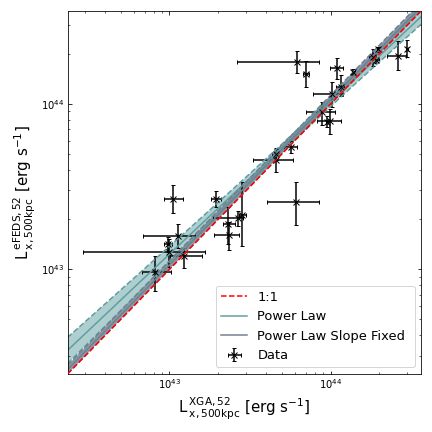
\includegraphics[width=0.95\columnwidth]{images/efeds_xcs_l500cal.png}
    \caption[]{Comparison of unabsorbed cluster luminosities within a 500kpc aperture, in the 0.5-2.0keV energy band, centered on eFEDS coordinates. Pale blue line indicates best fit power-law, with 68\% confidence levels given by shaded region. Grey line indicates a power-law fit with slope set to 1 (with 68\% confidence levels given by grey shaded region).}
    \label{fig:l500kpccomp}
\end{figure}

We use the \texttt{XGA} XSPEC \citep[][]{xspec} interface to measure spectroscopic properties of those clusters that have high enough quality data, and compare those values to those presented in the eFEDS data release. Note that we do not re-analyse the eFEDS data and compare purely to the measurements given by \cite{efedsclustercat}. We use \texttt{XGA} v0.2, SAS v17.0.0, and XSPEC v12.10.1.

\subsection{Fitting Procedure}
\label{subsec:fitproc}

Cluster spectra are extracted within a 500kpc fixed aperture (as the eFEDS catalogue contains a greater number of 500 kpc temperatures than 300 kpc) and centered on the eFEDS position.  Corresponding backgrounds are extracted within 1000-1500~kpc annuli. Non-cluster sources in both the 500kpc apertures and background regions are identified using the XCS region files, and their corresponding events are removed during spectrum generation.  We fit absorbed \cite[with tbabs, ][]{tbabs} plasma emission models \citep[APEC, ][]{apec} to the spectra; these models are standard for XCS analyses, but are also the same as those used in the eFEDS spectroscopic analysis. To maximise the similarity of our analysis to eFEDS we opt to use the abundance tables published by \cite{aspl} when performing our spectral fits. The abundance parameter of the APEC model in all cases is set to 0.3Z$_{\odot}$ and frozen, the nH parameter of the tbabs model is set from the full-sky HI survey by the \cite{nh} (using the HEASoft \texttt{nh} tool) and frozen. The redshift parameter is set to the eFEDS catalogue value and frozen.

% All available observations and cameras are allowed to contribute to the fit of a given galaxy cluster, provided that they meet certain conditions. First, we require every spectrum to have a minimum of 10 noticed channels, ensuring no spectra have been re-binned to have only one or two channels. Each of these spectra are first fit independently, with the temperature and normalisation parameters allowed to vary.  If the measured temperature is $\leq$0.01keV, $>$20keV, or the temperature uncertainty is $>$ 15keV, then the corresponding spectrum will be rejected and not included in the final fit. When a set of acceptable spectra has been compiled, a final simultaneous fit is performed using only those spectra. An absorbed plasma emission model is created for each spectrum, then the temperature and normalisation parameters of all models are linked.  For this fit we add a simple multiplicative constant, to account for the differences in normalisation from different observations and still allow us to retrieve a single normalisation value at the end (as it has a physical meaning). The constant of the first model is set to 1 and frozen, and in all other models is allowed to vary freely. Temperature values (after XSPEC has run a suitable error calculation step), as well as the un-absorbed luminosity in energy bands of our choice, are then determined from this final fit.

Observations and cameras that meet quality requirements contribute to the fit of a given galaxy cluster. Each spectrum is first fit independently, with the temperature and normalisation parameters allowed to vary. If the measured temperature is $\leq$0.01keV, $>$20keV, or the temperature uncertainty is $>$ 15keV, then the spectrum will not included be in the final fit. Then a final simultaneous fit is performed using only the accepted spectra. Temperature values and unabsorbed luminosities are then determined from this final fit. We will use a temperature measurement if, a) the measured temperature is less than 25~keV, b) the upper and lower uncertainties are both positive, and c) the larger uncertainty is less than three times the smaller. Luminosities will be used if the uncertainty is not greater than the value, and if the upper and lower uncertainties are both positive. If a cluster's temperature or luminosity measurement do not meet these requirements, they are excluded.

For a more complete explanation of the spectral fitting process and comparisons of results with other {\em XMM} analyses that confirm the veracity of measurements produced by this procedure, see \cite{xcsmassmethod}. All measurements for the eFEDS-XCS sample can be found in Table~\ref{tab:measurements}, along with eFEDS name, position, and redshift.

\begin{figure*}
    \centering
    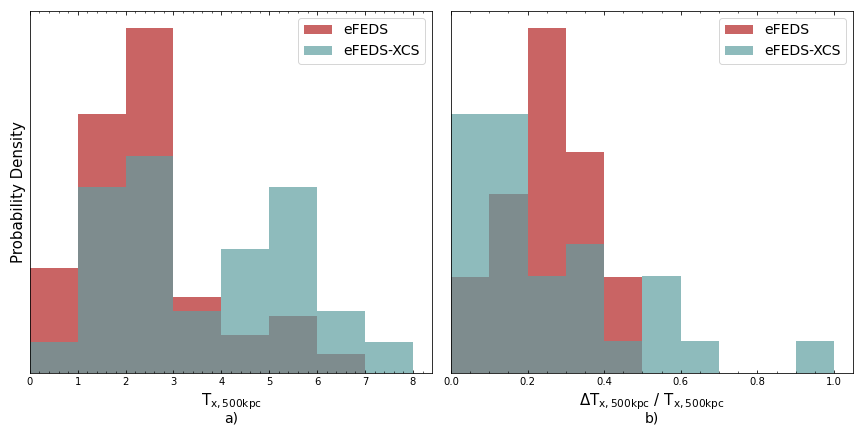
\includegraphics[width=1.0\textwidth]{images/efeds_xcs_txcomp.png}
    \caption[]{Temperature and fractional temperature error distributions of the eFEDS (red) and eFEDS-XCS (pale blue) samples, for measurements made within 500kpc apertures, centered on eFEDS coordinates. } 
    \label{fig:efedsxmmtxdist}
\end{figure*}

\subsection{Luminosity Comparison}
We compare the luminosities measured by both {\em XMM} and {\em eROSITA}, since one of the main products of {\em eROSITA} will be large catalogues of X-ray luminosities. These will be used as the basis of various {\em eROSITA} science applications, for example, a mass-luminosity scaling relation \citep[such as the one recently produced by ][]{efedsmor} provides a way to estimate overdensity radii of a given cluster, as well as enabling large scale X-ray cluster cosmology. Therefore, it is important to test the fidelity of eFEDS luminosities with {\em XMM} data. 

The eFEDS analysis presents cluster luminosities measured via a forward-fitting analysis of 2D count-rate maps, including considerations of the morphology of the cluster, rather than by the fitting of emission models to spectroscopic data. In the context of the eFEDS (and in the future eRASS), they are able to measure accurate luminosities for clusters that do not have high enough quality data to perform spectral fitting. As such, we can directly compare {\em XMM} and {\em eROSITA} luminosities for {\color{red} 29 (${\sim}$80\%)} of the eFEDS-XCS sample. We opt to use a spectral fitting process to measure unabsorbed (corrected for hydrogen column absorption) luminosities in the soft (0.5-2.0keV) and bolometric (0.01-100keV) energy bands for those clusters with a successful temperature measurement.

We fit the same two models as used for the temperature calibration (a power-law with the slope fixed at 1, and left to vary), to the luminosity comparison, finding the results of both to be entirely consistent with a one-to-one relation. Figure~\ref{fig:l500kpccomp} demonstrates an excellent soft-band luminosity agreement (including the two models) between eFEDS and XCS, especially considering how different the measurement methods are. Luminosities measured by eFEDS and XCS are similarly well constrained, though the XCS uncertainties tend to be slightly smaller. The bolometric luminosity comparison shows a similar agreement.

\subsection{Temperature Distributions Comparison}
We have been able to measure temperatures within a 500 kpc aperture for ${\sim}$80\% of the eFEDS-XCS sample, though only ${\sim}$30\% of those also have an eFEDS temperature available (see Table~\ref{tab:samples} for a summary). As such we first compare the overall temperature, and fractional temperature uncertainty, distributions, as we did in Section~\ref{sec:efedsproperties} with the XXL-100-GC sample.

Figure~\ref{fig:efedsxmmtxdist}a, which shows the overall temperature distributions of the eFEDS and eFEDS-XCS samples, demonstrates that a larger proportion of {\em XMM} temperatures than {\em eROSITA} temperatures are above ${\sim}$4~keV, similar to the behaviour in Figure~\ref{fig:xxlefeds}b with the XXL-100-GC sample. It is likely that this is due to the difference in telescope sensitivity at high energies, as well as other selection effects resulting from targeted {\em XMM} exposures, as previous work by \cite{xcsmethod} has shown that it is more difficult to measure temperatures for hotter galaxy clusters. Combined with the fact that we also observe this effect when eFEDS data is compared to XXL-100-GC, however, means that is another possible indication of a temperature calibration being required between the two telescopes. 

Figure~\ref{fig:efedsxmmtxdist}b demonstrates that a larger proportion of the eFEDS-XCS sample (compared to eFEDS measurements) have a fractional temperature uncertainty of less than 20\%, and as such the {\em XMM} temperature measurements are generally better constrained. However we also note that the temperature fractional error distribution of the eFEDS-XCS sample extends to larger values than eFEDS. 
% Although {\em XMM} has observed only a fraction of the total area of the sky, any cluster that does fall on a pointing (whether targeted or serendipitous) and can have an {\em XMM} temperature measured for it, is likely to have comparable constraints to an eFEDS temperature. However, especially for serendipitous clusters near the edge of the field of view, there will be instances were no temperature at all can be measured.

Archival {\em XMM} observations can provide temperatures which are, on average, better constrained than eFEDS for those clusters that have been observed by {\em XMM}, and can also deliver more temperatures for hotter systems due to {\em XMM}'s greater sensitivity at high energies.  As such the {\em XMM} archive will be a very useful complement to the eRASS.


\begin{figure}
    \centering
    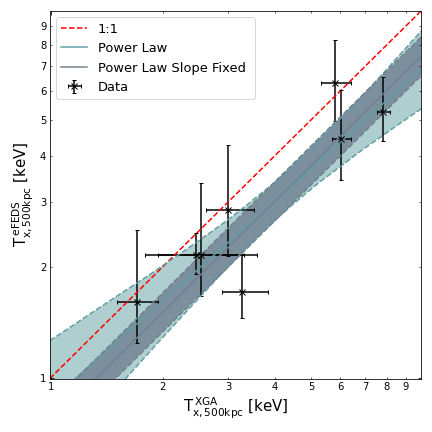
\includegraphics[width=0.95\columnwidth]{images/efeds_xcs_t500cal.png}
    \caption[]{Comparison of eFEDS and {\em XMM} cluster temperatures within 500kpc, centered on eFEDS coordinates. Pale blue line indicates best fit power-law, with 68\% confidence levels given by shaded region. Grey line indicates a power-law fit with slope set to 1 (with 68\% confidence levels given by the grey shaded region).}
    \label{fig:t500kpccomp}
\end{figure}

\subsection{Preliminary Temperature Calibration}
\label{subsec:tcal}
We must test for a difference in temperatures measured by {\em XMM} and {\em eROSITA}, so our first comparison is made between temperatures presented in the eFEDs cluster catalogue and {\em XMM} temperatures that we have measured for the same clusters. 

A comparison of the 8 clusters with measured {\em XMM} and eFEDS temperatures is given in Figure~\ref{fig:xmmexposure} that appears to show a systematic offset between the two telescopes.  All but one of the clusters are below the one-to-one line, indicating that the {\em XMM} temperatures are systematically higher than the {\em eROSITA} temperatures. The majority of eFEDS temperatures are consistent with the one-to-one line, but not the temperatures measured from {\em XMM} data, as they are generally better constrained (a behaviour we saw in Figure~\ref{fig:efedsxmmtxdist}). To model this, we fit a power law of the form

\begin{align}
{\rm log}\left(T^{\:\rm{eROSITA}}_{\rm{x, 500kpc}}\right) &= {\rm log}(A_{TT}) + B_{TT}{\rm log}\left(T^{\:\rm{XMM}}_{\rm{x, 500kpc}}\right) \pm \sigma_{T_{\rm{eROSITA}}|T_{\rm{XMM}}},
\label{equ:TvsT}
\end{align}
where $A_{TT}$ is the normalisation, $B_{TT}$ the slope and $\sigma_{T_{\rm{eROSITA}}|T_{\rm{XMM}}}$ the intrinsic scatter. The fits were performed in log space using the R package LInear Regression in Astronomy\citep[{\sc lira}\footnote{\href{https://cran.r-project.org/web/packages/lira/index.html}{LInear Regression in Astronomy}}, ][]{softlira}, fully described in \cite{LIRA}. The best fit parameters are given in Table~\ref{tab:tempcal}. 

First, we fit the power law with the slope left free to vary, probing whether the observed offset evolves with temperature \citep[as found in][comparing between {\em Chandra} and {\em XMM}]{xmmchandracal}. We measure a slope value of 0.87$^{+0.37}_{-0.27}$, indicating that the calibration evolves with system temperature.  We note however that due to the large errors, the value of $B_{TT}$ is consistent with 1 (within 1$\sigma$).  The measured intrinsic scatter of both fits is very low (essentially consistent with zero), which is as expected.
 
Due to the large errors on the measure slope, we re-fit the power-law with the slope fixed at unity.  This allows us to measure a single overall factor that describes the average difference in temperatures measured by the two telescopes.  We measure a normalisation of 0.75$^{+0.09}_{-0.08}$, meaning that (on average) {\em eROSITA} measures a temperature ${\sim}25\%$ cooler than those measured by {\em XMM} for the same cluster.

\begin{table}
\begin{center}
\caption[]{{\small The normalisation, slope, and intrinsic scatter values of the fitted temperature calibration models for 500kpc apertures. $A_{TT}$ is normalisation, $B_{TT}$ is slope, and $\sigma_{T_{\rm{eROSITA}}|T_{\rm{XMM}}}$ the intrinsic scatter.}\label{tab:tempcal}}
\vspace{1mm}
\begin{tabular}{cccc}
\hline
\hline
Calibration Name & $A_{TT}$ & $B_{TT}$ & $\sigma_{T_{\rm{eROSITA}}|T_{\rm{XMM}}}$\\
\hline
\hline
Power Law & $0.90^{+0.24}_{-0.24}$ & $0.87^{+0.37}_{-0.27}$ & $0.04^{+0.06}_{-0.04}$ \\
\hline
Power Law Fixed Slope & $0.75^{+0.09}_{-0.08}$ & $1$ & $0.04^{+0.05}_{-0.02}$ \\
\hline
\end{tabular}
\end{center}
\end{table}

As we have not re-analysed {\em eROSITA} spectra and measured our own temperatures for the eFEDS-XCS cluster sample, our methodologies are unlikely to be completely consistent, and as such the observed temperature calibration could be the result of some mismatch in our measuring procedures. This calibration fit is also affected by small number statistics, as very few clusters have both an eFEDS and an {\em XMM} temperature. However, we have provided evidence of an offset that requires further investigation.


\section{Discussion}
\label{sec:discussion}
In this work we have presented a measurement of the temperature offset between {\em eROSITA} and {\em XMM} for a sample of galaxy clusters.  Here we discuss potential impacts of this offset on the derived scaling relations and how the temperature calibration can be improved.  Furthermore, we explore differences in the measured centroids for eFEDS and XCS clusters and the impact on miscentering calibration on optical cluster finders.

\subsection{{\em\lower{e}ROSITA}-{\em XMM} Temperature Calibration}
\begin{figure}
    \centering
    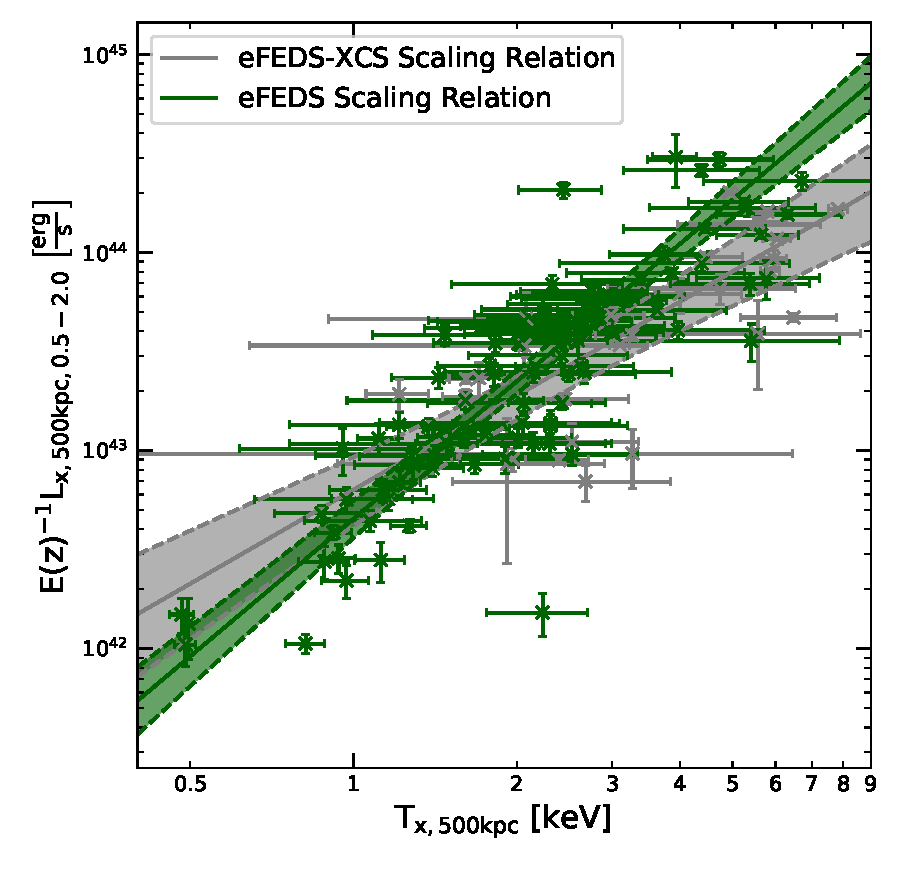
\includegraphics[width=1\columnwidth]{images/efeds_xcs_wdata_lt52.pdf}
    \caption[]{Soft-band luminosity-temperature relations for the eFEDS and eFEDS-XCS samples. Properties measured within a 500kpc fixed aperture centered on the eFEDS positions.}
    \label{fig:efedsandxcslt}
\end{figure}

\subsubsection{Luminosity-Temperature Relation}
\label{subsubsec:LT}
Considering the temperature offset measured in Section~\ref{subsec:tcal}, we must ascertain the impact on any  derived scaling relations, especially when comparing between telescopes.  We focus on the luminosity-temperature relation derived from eFEDS and XCS data.  This relation is frequently used to probe the self-similarity of a population of clusters, but in this case we wish to use it as a diagnostic tool to probe differences in measurements made by eFEDS and XCS.  We use all eFEDS-XCS clusters with a successful 500~kpc temperature ($T^{\rm 500kpc}_{\rm X}$) and soft-band luminosity ($L^{\rm 500kpc}_{X,0.5-2.0}$) measurement (instead of the of the 8 clusters used for the temperature calibration, due to small sample size), and all available eFEDS candidates and compare the relations.  

The L$^{500\rm{kpc}}_{\rm{X,0.5-2.0}}$ - T$_{\rm{X}}^{500\rm{kpc}}$ relation for eFEDS (grey point) and eFEDS-XCS (green points) is shown in Figure~\ref{fig:efedsandxcslt}, using data from 94 (eFEDS) and 29 (eFEDS-XCS) galaxy clusters.  The data cover a similar temperature range (see Figure~\ref{fig:efedsxmmtxdist}), ensuring the eFEDS-XCS sample does not preferentially select a particular population of high or low temperature clusters, and as such it is valid to compare eFEDS-XCS and eFEDS luminosity-temperature relations directly.  We fit both datasets using a power law of the form, 
\begin{align}
{\rm log}\left(\frac{L^{500\rm{kpc}}_{\rm{X,0.5-2.0}}}{E(z)L_{0}}\right) &= {\rm log}(A_{LT}) + B_{LT}{\rm log}\left(\frac{T^{\rm{500kpc}}_{\rm{X}}}{T_{0}}\right) \pm \sigma_{L|T},
\label{equ:lt}
\end{align}
where $A_{LT}$ denotes the normalisation, $B_{LT}$ the slope, and $\sigma_{L|T}$ the intrinsic scatter of the relation. We calculate E(z) using the redshift supplied in the eFEDS catalogue and our chosen concordance cosmology.  The fits are again performed using the LIRA package. We set the normalisation values for soft-band luminosity and temperature to approximate median eFEDS values of $L_{0}$=2.0$\times$10$^{43}$~erg~s$^{-1}$ and $T_{0}$=2.3~keV.

Figure~\ref{fig:efedsandxcslt} shows the best-fit relations  using the eFEDS (green line) and eFEDS-XCS (grey line) samples respectively.  The best-fit values are given in Table~\ref{tab:relations}, with their distributions illustrated in Figure~\ref{fig:ltcorner}.  While the distributions highlight that the parameters of the relation are consistent within their 2$\sigma$ contours, the difference in the central value of the slope is investigated further.  We explore whether this difference can be reduced based upon the observed temperature offset found in Section~\ref{subsec:tcal}.

\begin{figure}
    \centering
    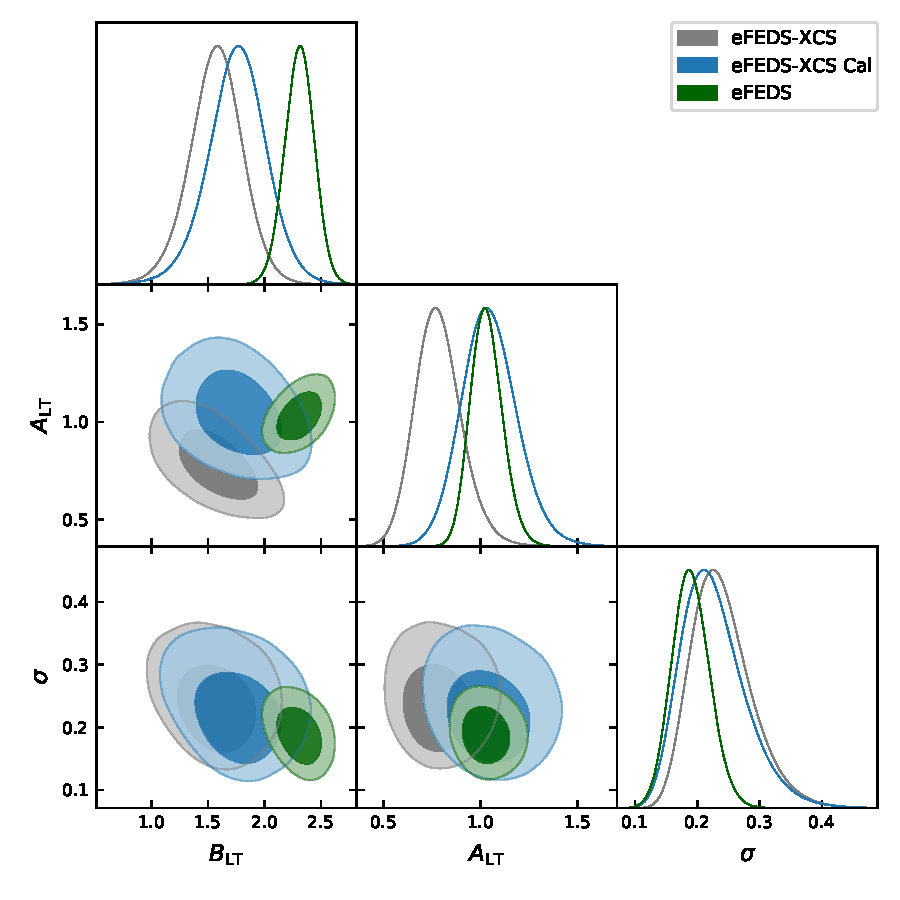
\includegraphics[width=1\columnwidth]{images/lt52_corner.pdf}
    \caption[]{Corner plot of the 1$\sigma$ and 2$\sigma$ confidence contours of the L$^{500\rm{kpc}}_{\rm{x, 0.5-2.0}}$ - T$^{500\rm{kpc}}$ relation parameters, for the eFEDS (green contours), eFEDS-XCS (grey contours) and eFEDS-XCS calibrated (blue contours) samples.  The diagonal shows the posterior densities of each parameter.}
    \label{fig:ltcorner}
\end{figure}

\begin{figure}
    \centering
    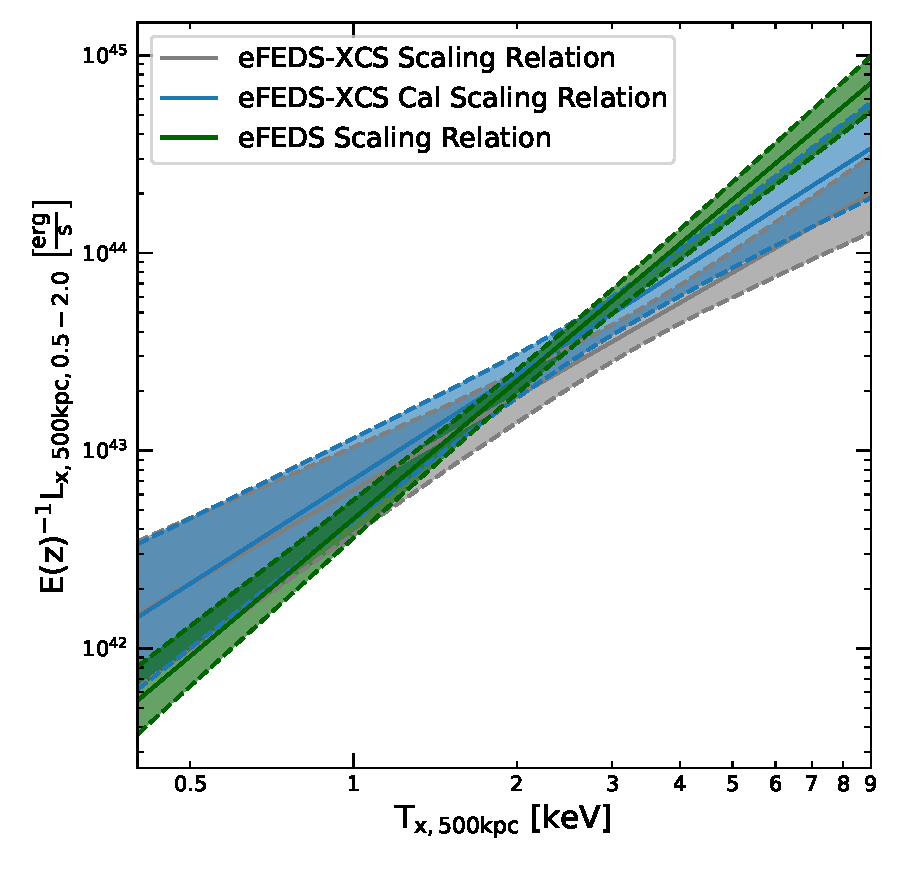
\includegraphics[width=1\columnwidth]{images/efeds_lt52.pdf}
    \caption[]{Soft-band luminosity-temperature relations for eFEDS, eFEDS-XCS, and calibrated eFEDS-XCS. Properties measured within a 500kpc fixed aperture centered on the eFEDS positions.}
    \label{fig:prelimlt}
\end{figure}

\begin{table}
\begin{center}
\caption[]{{\small The normalisation, slope, and residual scatter values from the LIRA fits of the different datasets, for the L$^{500\rm{kpc}}_{\rm{x, 0.5-2.0}}$ - T$_{\rm{x}}^{500\rm{kpc}}$ scaling relation.}\label{tab:relations}}
\vspace{1mm}
\begin{tabular}{cccc}
\hline
\hline
Relation Name & $A_{LT}$ & B_{LT} & \sigma_{L|T}\\
\hline
\hline
eFEDS & $1.54^{+0.13}_{-0.12}$ & $2.31^{+0.13}_{-0.13}$ & $0.19^{+0.03}_{-0.03}$ \\
\hline
eFEDS-XCS & $1.18^{+0.19}_{-0.17}$ & $1.57^{+0.22}_{-0.23}$ & $0.23^{+0.05}_{-0.04}$ \\
\hline
eFEDS-XCS Calibrated & $1.57^{+0.22}_{-0.20}$ & $1.74^{+0.24}_{-0.25}$ & $0.23^{+0.06}_{-0.05}$ \\
\hline
\end{tabular}
\end{center}
\end{table}

% \subsection{Measuring a calibrated eFEDS-XCS relation}

% Finally, we measure a third version of the scaling relation, designed to test the effect of the temperature calibration we quantify in section \ref{subsec:tcal} on the full eFEDS-XCS sample. If a calibration is required between temperatures measured by {\em eROSITA} and {\em XMM}, then we would expect to see differences in the normalisation and slope of luminosity-temperature relations created from the two instruments. The two cases we consider in our efforts to quantify the observed temperature discrepancy (a constant factor, or relation that evolves with T$_{x}$ would produce different effects in a luminosity-temperature relation. A constant factor temperature offset would only have a significant effect on the normalisation of the relation, whereas an evolving offset would also have an impact on the slope. Figure \ref{fig:efedsandxcslt} makes it quite clear that there are significant differences in the slopes of the two relations, which better fits the second case, an evolving temperature calibration. As such, we measure the calibrated luminosity-temperature relation by using the power law model (with slope free to vary), with parameter values provided in Table~\ref{tab:tempcal}, to simply convert the valid eFEDS-XCS temperature values to their equivalent eROSITA values. 

% Unfortunately, as they are built upon a population, scaling relations are sensitive to selection effects and as such our comparison of eFEDs, eFEDS-XCS, and calibrated eFEDS-XCS scaling relations may be affected (unlike our direct temperature comparison). However, if we measure the relation with a calibration applied to {\em XMM} temperatures and it brings the eFEDS and eFEDS-XCS relations into better agreement with one another, it could still be another hint that such a calibration is required. 

% \subsubsection{Comparison of relations}
Therefore, we measure a third version of the scaling relation, designed to test the effect of the temperature calibration quantified in Section \ref{subsec:tcal}.  We determine a ``calibrated'' luminosity-temperature relation by using the power law model (with slope free to vary), with parameter values provided in Table~\ref{tab:tempcal}, to simply convert the valid eFEDS-XCS temperature values to their equivalent eROSITA values.

Figure~\ref{fig:prelimlt} shows the model fits for all three relations (with data points omitted for clarity), and shows that the eFEDS-XCS calibrated scaling relation has a steepened slope and increased normalisation when compared to the original eFEDS-XCS relation.  Figure~\ref{fig:ltcorner} shows a shift of the contours and distributions (the eFEDS-XCS calibrated parameters are given by the blue contours) towards eFEDS (blue contours).  The normalisation of the calibrated eFEDS-XCS relation is fully consistent with the eFEDS relation, with the tension in the measured slopes reduced.  

While the eFEDS-XCS calibrated relation shifts towards the overall eFEDS relation, the remaining difference could be related to the small number of clusters used to measure the calibration function or selection effects, but this comparison could be another indication of a temperature disparity between {\em XMM} and {\em eROSITA}.

%The luminosity temperature relations presented in Table~\ref{tab:relations} were measured for these comparisons rather than a scientific use-case, as using a fixed aperture for luminosity measurements in that context would not be valid; as such we choose not to compare to existing scaling relations in literature.

\subsubsection{Mass-Observable Relations}
We must also consider the impact of the temperature offset on any mass-observable relations constructed, or used by, the {\em eROSITA} collaboration. Where {\em eROSITA} analyses are self-contained the offset will have no effect, its only when data from {\em XMM} is required, or when an {\em eROSITA} relation is used for {\em XMM} analysis, that it must be considered. The eRASS will be able to produce well constrained mass-temperature relations \citep[e.g.,][using eFEDS data]{efedsmor}, which are likely to be used in analyses involving other telescopes; for this to be possible we must have a good understanding of the temperature calibration.

Though it is unlikely that any hydrostatic masses will be measured from eRASS data (such a measurement requires more X-ray counts than the relatively short exposure time of eRASS will collect), they may still be of interest to the {\em eROSITA} team. This method produces masses of individual clusters, rather than a stack, and as such mass-observable relations generated with hydrostatic masses retain useful information about the scatter. As such, it is possible that {\em XMM} hydrostatic mass-temperature relations will be incorporated into {\em eROSITA} work, and if this is the case then the temperature offset must be quantified well enough to convert {\em XMM} temperatures to {\em eROSITA} equivalents. Once the eRASS is complete, {\em eROSITA} will be used for pointed observations, from which hydrostatic masses can be calculated (\cite{pointysanders} measured the mass of Abell 3266 during {\em eROSITA} commissioning), at which point a hydrostatic mass-temperature relation might be generated; again an understanding of the calibration will be required for {\em XMM} analyses to make use of such a relation.

\begin{figure*}
    \centering
    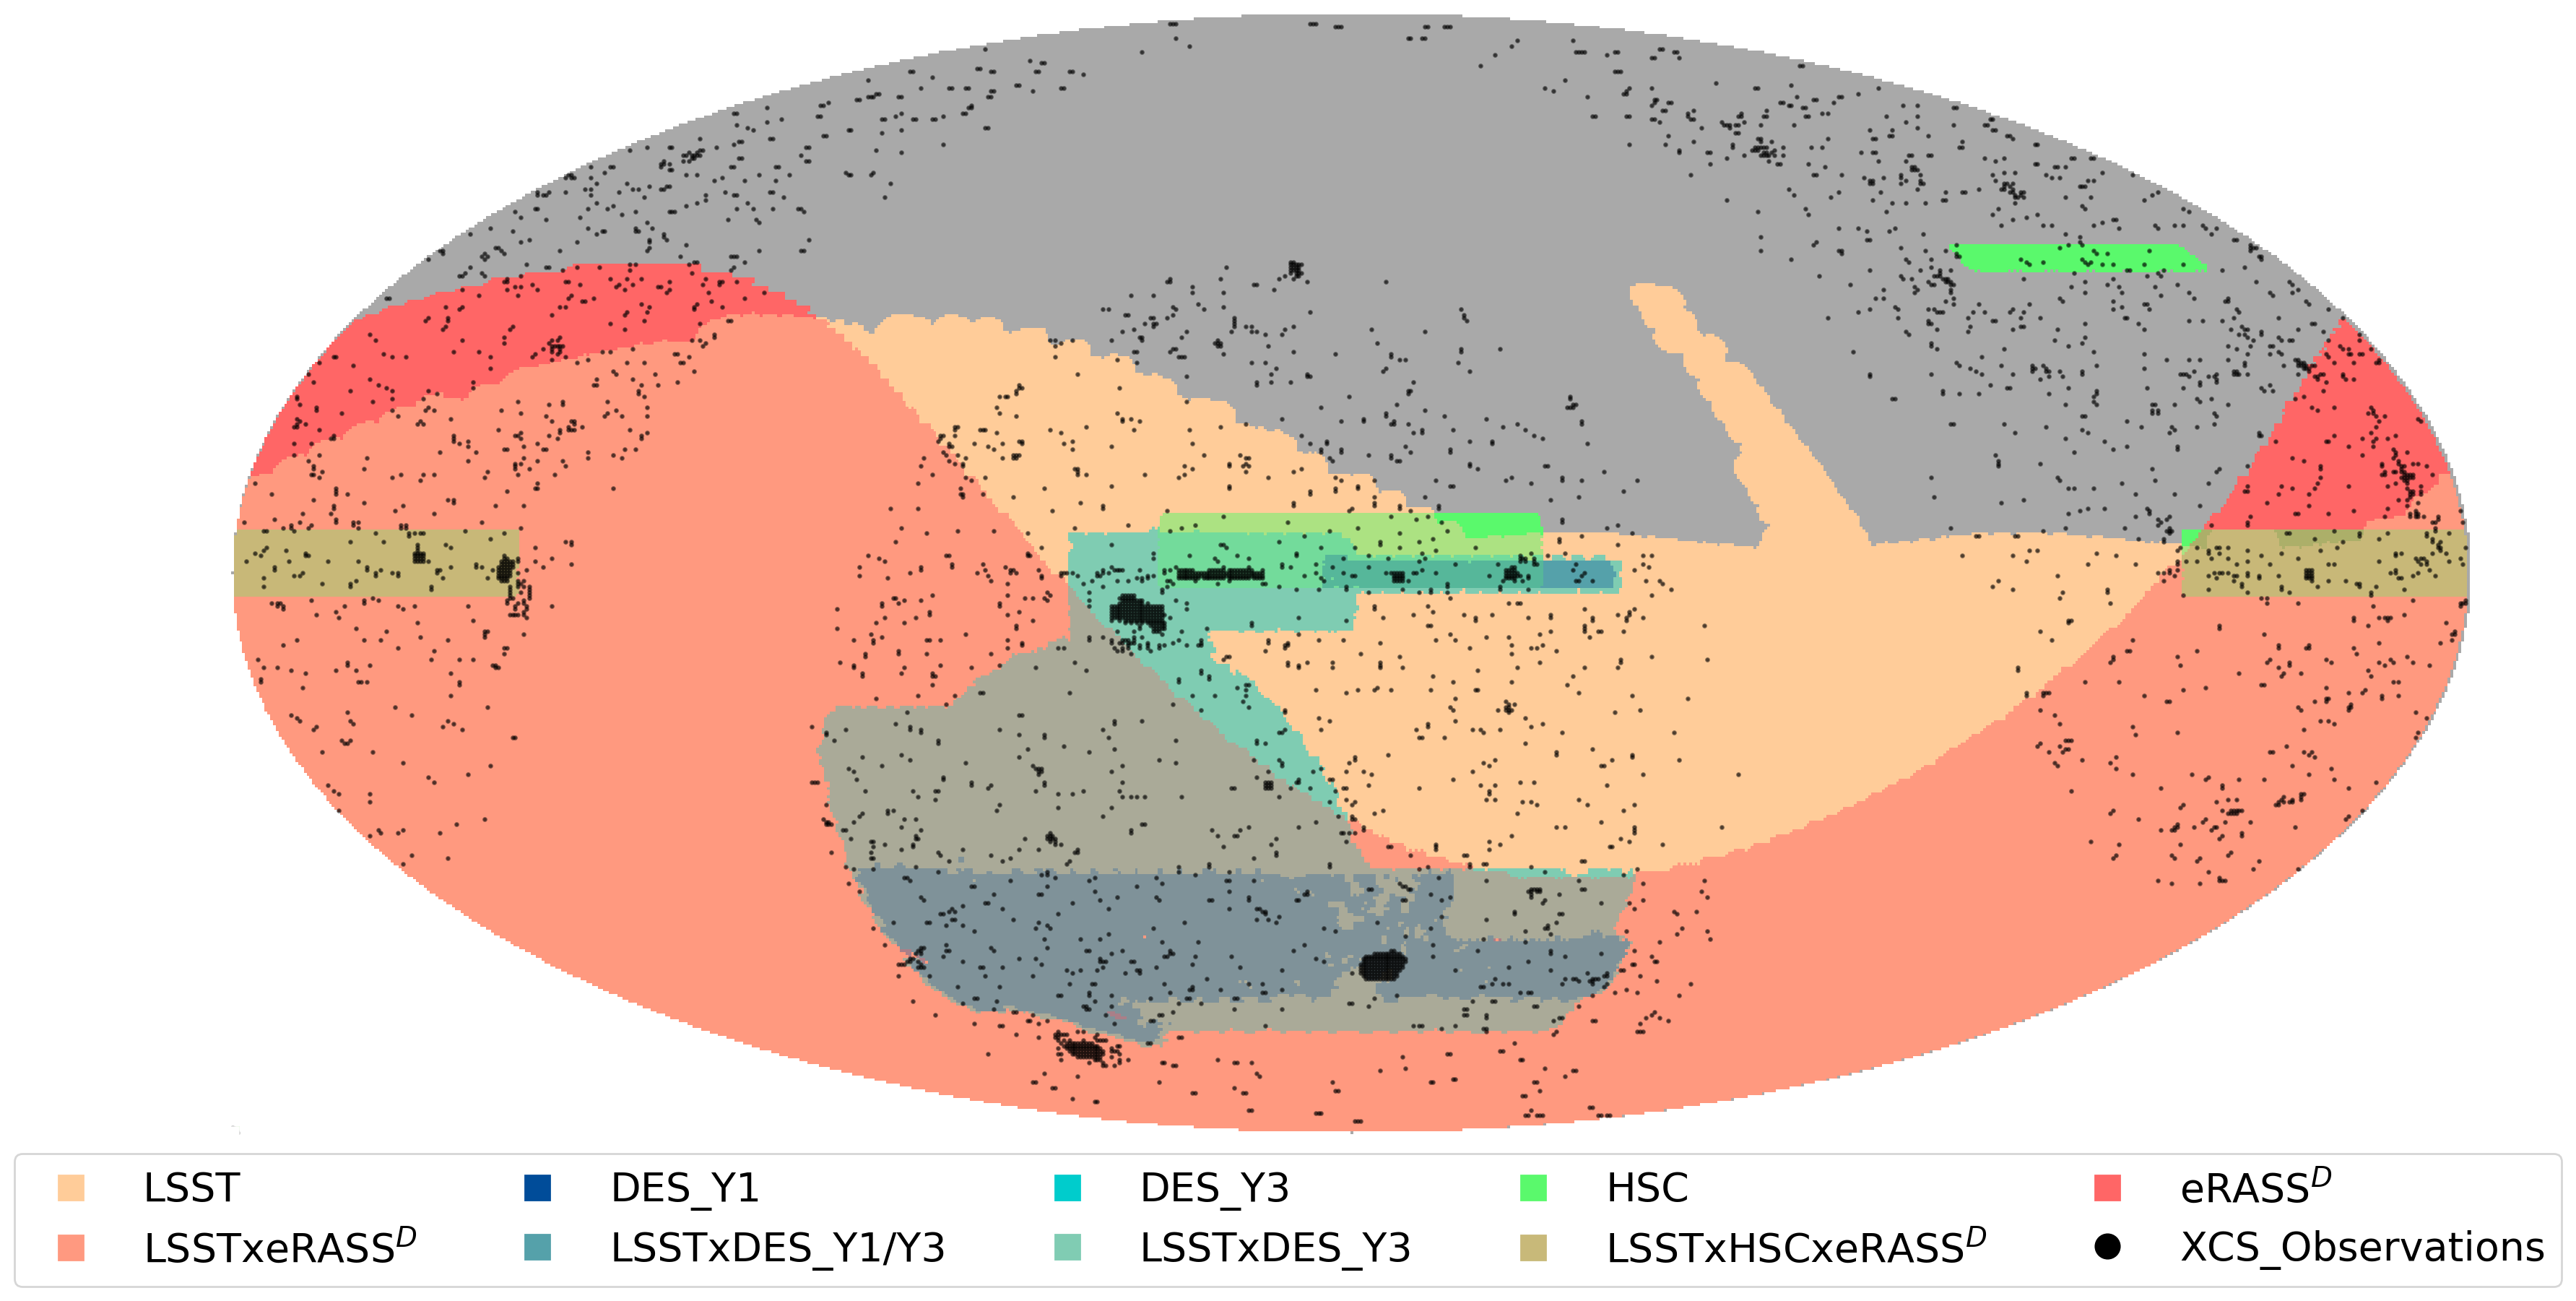
\includegraphics[width=0.98\textwidth]{images/xmm_erass_footprint.png}
    \caption[]{{\color{red} PLACEHOLDER} Distribution of {\em XMM} observations projected over the sky, indicated by {\color{red} black} regions. eRASS (German) highlighted by the {\color{red} orange} region.} 
    \label{fig:germanerassxmm}
\end{figure*}

\subsubsection{Improving the Calibration}
Aspects of our work motivate further exploration of the temperature comparison between the {\em XMM} and {\em eROSITA} telescopes, most importantly the observed temperature offset in Section~\ref{subsec:tcal} and the luminosity-temperature relations in Section~\ref{subsubsec:LT}. This is because a detailed understanding of the temperature offset is crucial for any cross-telescope analysis between {\em XMM} and {\em eROSITA}, and the calibrations in Table~\ref{tab:tempcal} do not fully correct the differences between the {\em XMM} and {\em eROSITA} luminosity-temperature relations in Figure~\ref{fig:prelimlt}.

There are several ways in which we can improve our understanding of the calibration. Firstly, a complete re-analysis of the eFEDS cluster candidates' raw data using an identical methodology to the {\em XMM} analysis is required; this will eliminate a possible cause of the temperature discrepancy seen in Figure~\ref{fig:t500kpccomp}. This will also allow us access to the temperatures that were not published as part of the eFEDS catalogue due to being poorly constrained. 

Secondly, to better constrain the relationship between {\em XMM} and {\em eROSITA} temperatures we should also aim to acquire follow-up {\em XMM} observations of a representative sample of eFEDS cluster candidates, preferentially targeting optically confirmed systems with the best temperature constraints of the sample. Both increasing the size of the sample that we can directly compare to, and comparing to clusters that have better constrained temperatures, will reduce the uncertainties on our temperature calibration model. This will be especially helpful for better constraining the slope of the calibration, and when combined with a re-analysis of eFEDS will give a better description of the temperature calibration.

Thirdly, the eRASS survey will greatly increase the scope for direct temperature comparisons with {\em XMM} observed galaxy clusters, as it will take data for every {\em XMM} cluster. The data sharing agreement between the German and Russian consortiums that funded {\em eROSITA} involves sharing the sky equally, and the {\em eROSITA}-DE team have provided a data release schedule\footnote{\href{https://erosita.mpe.mpg.de/erass/}{{\em eROSITA}-DE Data Release Schedule}}. Figure~\ref{fig:germanerassxmm} demonstrates that the {\em eROSITA}-DE data intersect with many {\em XMM} observations, meaning that there is significant scope for comparisons of {\em XMM} and {\em eROSITA} observed galaxy clusters. The first German eRASS data release (with two passes of their half of the sky) is due in Q4 2022, and as such will not be available to the general community for at least a year. It will also not be full-depth (as the eFEDS is); that means temperatures will in general be less well constrained. Poorer constraints will be offset by the number of temperatures available, but this approach to the improvement of the temperature calibration will be most effective when used in concert with targeted {\em XMM} follow-up.

\subsection{Positions of cluster central coordinates}
We observed some cases where the eFEDS coordinate deviates significantly from that of a matching XAPA extended source. This generally seems to be due low signal-to-noise {\em eROSITA} data for that cluster candidate, though in some cases point source contamination appears to shift the central coordinate toward the point source. This could cause issues when combining eRASS and optical cluster catalogues, as X-ray observations are often used to calibrate the mis-centering of optical cluster finders \citep[][]{desmiscentering}, which often select the BCG as the central coordinate. Creating mis-centering priors from eRASS catalogues may be difficult if there is a large proportion of poorly constrained central coordinates.

\begin{figure}
    \centering
    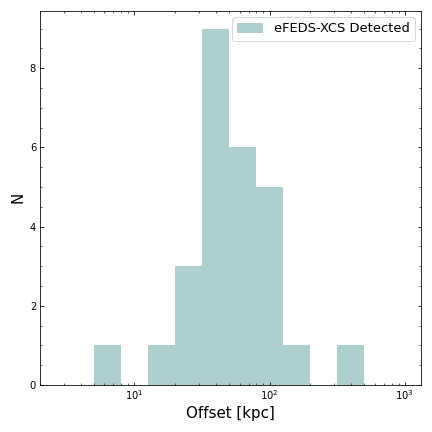
\includegraphics[width=0.95\columnwidth]{images/eFEDS_XAPA_offset.png}
    \caption[]{Comparison of eFEDS central coordinates to XAPA central coordinates, for the subset of the eFEDS-XCS sample that have been detected by XAPA.}
    \label{fig:centcoords}
\end{figure}

We compare the eFEDs positions of eFEDS-XCS clusters to XAPA detection central coordinates for those clusters that have been detected by XCS.  Figure~\ref{fig:centcoords} plots the distributions of offsets between the eFEDS and XAPA coordinates (in units of kpc, calculated at the eFEDS redshift).  This indicates that there can be significant differences in the centroid positions of the two surveys, though the majority of the clusters have an offset smaller than 100kpc. We chose XAPA central coordinates rather than \texttt{XGA} peak positions to provide the fairest comparison for eFEDS positions, as centroid and peak finder techniques for measuring a central cluster position differ significantly.  We also expect centroid techniques to perform better on shallower data, though X-ray peaks are preferred for calibrations of mis-centering. 


\section{Summary}
\label{sec:summary}

In this work we have performed the first comparison between cluster properties measured by the eFEDS survey and those measured by {\em XMM} surveys, such as XCS and XXL, both directly and for whole cluster populations. We have located and analysed eFEDS cluster candidates which have a counterpart in an {\em XMM} observation, and presented comparison's between cluster temperatures and luminosities. As part of this process we also visually inspected the eFEDS cluster candidates that lie on an {\em XMM} observation and rejected any that had no ICM emission at the eFEDS coordinates, had obviously contaminated ICM emission, or too low quality {\em XMM} data.

A discrepancy between cluster temperatures measured by eFEDS and XCS has been found and quantified, which could hint at the need for a calibration function between the eROSITA and {\em XMM} telescopes (as has been necessary between {\em XMM} and {\em Chandra}). Several variables need to be better controlled before we can definitively state that the observed discrepancy is entirely due to a required temperature calibration, but combined with the enhanced fraction of higher temperature clusters in the XXL-100-GC and eFEDS-XCS catalogues when compared to eFEDS values, we consider it to be a likely explanation. 
 
Our analysis finds excellent agreement between soft-band luminosities measured by eFEDS and \texttt{XGA} for the eFEDS-XCS sample, which is very encouraging for future eRASS cosmology analyses. Such analyses will rely almost exclusively on mass-luminosity relations \citep[such as the eFEDS-HSC collaboration, ][]{efedsmor}, as even full depth eRASS will not be able to measure temperatures for enough galaxy clusters. 

We also fit and compare the first luminosity-temperature scaling relations using data from eFEDS and eFEDS-XCS {\em XMM} counterparts, using them to compare scaling relations measured with {\em eROSITA} and {\em XMM} data. This has particular relevance for anyone wishing to use an {\em XMM} generated scaling relation in an {\em eROSITA} analysis, or vice versa, as we find a distinct tension between scaling relations from the eFEDS and eFEDS-XCS samples. We also generate a second, calibrated, eFEDS-XCS scaling relation which is in slightly better agreement with the eFEDS relation, which again may suggest that a temperature scaling between {\em XMM} and {\em eROSITA} is necessary. It is likely, however, that a large part of the observed tension between the scaling relations is due to selection effects.

Our visual inspections of the eFEDS cluster candidates that fall on an {\em XMM} field (using {\em eROSITA}, {\em XMM}, and SDSS images) have shown that there are some aspects of {\em eROSITA}'s source finding and confirmation steps that can introduce spurious sources into their catalogues, which in turn could impact their cosmological analyses. Our inspection process finds that the eFEDS-XMM sample is ${\sim}$24\% contaminated (broadly in line with eFEDS predictions and measured values), and that only a minimal (${\sim}$3\%) level of contamination remains in the optically confirmed sample.

Our comparisons have shown that we can expect a great deal of useful data from the full eRASS catalogues, and that {\em XMM}-Newton still has a significant part to play as followup instrument. Its archive of 20 years worth of observations is still extremely valuable to the {\em eROSITA} team, and the X-ray astronomy community as a whole, and there will be many excellent opportunities for synergies between the two telescopes.

% A full examination of {\em eROSITA} and SDSS images generated around the positions of every eFEDS cluster candidate is required to understand how often X-ray source detection issues arise in a full eRASS depth field, as the eFEDS-{\em XMM} sub-sample may not be representative of the number of issues found in the full field. Given the scale of eRASS, and the number of clusters it expects to find, it is unfeasible to have a human visually examine every candidate. As such it is crucial that the eFEDS field is used to understand whether some of the contamination of the X-ray sample can be offset by extra diagnostic steps or techniques.

% An analysis working in the other direction, taking XCS cluster candidates and searching for their counterparts in the eFEDS field, to understand the detection limits of eFEDS and if/why it misses clusters detected in {\em XMM} observations by XCS.

\section*{Acknowledgements}
This work is based on data from eROSITA, the soft X-ray instrument aboard SRG, a joint Russian-German science mission supported by the Russian Space Agency (Roskosmos), in the interests of the Russian Academy of Sciences represented by its Space Research Institute (IKI), and the Deutsches Zentrum für Luft- und Raumfahrt (DLR). The SRG spacecraft was built by Lavochkin Association (NPOL) and its subcontractors, and is operated by NPOL with support from the Max Planck Institute for Extraterrestrial Physics (MPE). The development and construction of the eROSITA X-ray instrument was led by MPE, with contributions from the Dr. Karl Remeis Observatory Bamberg & ECAP (FAU Erlangen-Nuernberg), the University of Hamburg Observatory, the Leibniz Institute for Astrophysics Potsdam (AIP), and the Institute for Astronomy and Astrophysics of the University of Tübingen, with the support of DLR and the Max Planck Society. The Argelander Institute for Astronomy of the University of Bonn and the Ludwig Maximilians Universität Munich also participated in the science preparation for eROSITA.

The eROSITA data shown here were processed using the eSASS software system developed by the German eROSITA consortium.

We made frequent use of TOPCAT \citep[][]{topcat} during the initial exploration of the eRASS cluster catalogue.

The new X-ray analysis module developed by XCS (XGA) makes significant use of Astropy \citep[][]{astropy1, astropy2}, NumPy \citep[][]{numpy}, Matplotlib \citep[][]{matplotlib}, and pandas \citep[][]{pandassoftware,pandaspaper}. XGA also uses GetDist \citep[][]{getdist} to produce corner plots.

DT, KR, and PG acknowledge support from the UK Science and Technology Facilities Council via grants {\color{red}***} (DT), {\color{red}***} (KR, PG).
%%%%%%%%%%%%%%%%%%%%%%%%%%%%%%%%%%%%%%%%%%%%%%%%%%
\section*{Data Availability}

The data underlying this article were accessed from the \href{https://erosita.mpe.mpg.de/edr/eROSITAObservations/Catalogues/}{eROSITA Early Data Release site}. The data underlying this article are available in the article and in its online supplementary material.

%%%%%%%%%%%%%%%%%%%% REFERENCES %%%%%%%%%%%%%%%%%%

% The best way to enter references is to use BibTeX:

\bibliographystyle{mnras}
\bibliography{xcs_efeds} % if your bibtex file is called example.bib


% Alternatively you could enter them by hand, like this:
% This method is tedious and prone to error if you have lots of references
%\begin{thebibliography}{99}
%\bibitem[\protect\citeauthoryear{Author}{2012}]{Author2012}
%Author A.~N., 2013, Journal of Improbable Astronomy, 1, 1
%\bibitem[\protect\citeauthoryear{Others}{2013}]{Others2013}
%Others S., 2012, Journal of Interesting Stuff, 17, 198
%\end{thebibliography}

%%%%%%%%%%%%%%%%%%%%%%%%%%%%%%%%%%%%%%%%%%%%%%%%%%

%%%%%%%%%%%%%%%%% APPENDICES %%%%%%%%%%%%%%%%%%%%%

% \newpage
\appendix

\section{Excluded Cluster Candidates}
\label{app:rejected}

This section details the eFEDS-{\em XMM} X-ray cluster candidates that were dropped from our final sample, as discussed in Section \ref{sec:efedsxmm}. Table~\ref{tab:xmmrejects} contains candidates that were not included due to the low quality of the {\em XMM} data available, Table~\ref{tab:contamrejects} contains candidates that were rejected from our final sample (see Sect.~\ref{sec:efeds-varification}).

\begin{table*}
\begin{center}
\caption[]{{eFEDS-{\em XMM} galaxy cluster candidates dropped due to {\em XMM}-Newton data quality issues.}\label{tab:xmmrejects}}
\vspace{1mm}
\begin{tabular}{lccc|l}
\hline
\hline
eFEDS Name & ID & RA & Dec & Reason for Dropping\\
\hline
\hline
eFEDS J085434.6-014038 & 8094 & 133.644 & -1.677 & Dropped due to being on the edge of the {\em XMM} detector \\ 
\hline 
eFEDS J085440.5-020931 & 7700 & 133.669 & -2.159 & Dropped due to being on the edge of the {\em XMM} detector \\ 
\hline
eFEDS J085530.2-010634 & 1797 & 133.876 & -1.11 & Dropped due to being on the edge of the {\em XMM} detector appears to be a cluster in eFEDS \\ 
\hline 
eFEDS J090105.3-012525 & 11836 & 135.272 & -1.424 & Dropped due to being on the edge of a shallow {\em XMM} observation appears to be extended in eFEDS \\ 
\hline 
eFEDS J090409.7+003831 & 8977 & 136.04 & 0.642 & XMM observation appears to be badly affected by flaring \\ 
\hline
eFEDS J085901.6+010649 & 2757 & 134.756 & 1.114 & Matches to an XCS point source, but data is too low quality to use \\
\hline
eFEDS J090644.8+011124 & 5858 & 136.687 & 1.19 & Appears to be a cluster based upon eFEDS image, however, {\em XMM} data too shallow to confirm cluster \\
\hline
eFEDS J090752.9+013407 & 2074 & 136.971 & 1.569 & Candidate detected as an XCS point source. {\em XMM} data too poor to confirm, deny, or analyse\\ 
\hline 
eFEDS J091248.3+002446 & 11837 & 138.201 & 0.413 & {\em XMM} observation is affected by flaring but there appears to be no source in eFEDS \\ 
\hline 
\end{tabular}
\end{center}
\end{table*}

\begin{table*}
\begin{center}
\caption[]{{eFEDS-{\em XMM} galaxy cluster candidates rejected during our visual inspection.\newline $^\dagger$ indicates that the candidate was present in the optically confirmed sample from \cite{efedsclusteropticalcat}.}\label{tab:rejects}}
\vspace{1mm}
\begin{tabular}{lccc|l}
\hline
\hline
eFEDS Name & ID & RA & Dec & Reason for Rejection\\
\hline
\hline
eFEDS J084135.0+010150$^\dagger$ & 1644 & 130.396 & 1.031 & XCS detects two point sources from a targeted observation of an interacting galaxy pair with nuclear activity \\ 
\hline 
eFEDS J084201.8+005942$^\dagger$ & 3334 & 130.508 & 0.995 & No obvious source of any kind at coordinates especially at the redshift of 0.087 supplied by eFEDS catalogue \\ 
\hline
eFEDS J085022.3+001607$^\dagger$ & 8602 & 132.593 & 0.269 & This candidate is a cluster that has been split in two the other part is eFEDS J085027.9+001503 \\ 
\hline 
eFEDS J085255.2-013737$^\dagger$ & 1376 & 133.23 & -1.627 & No obvious source of any kind at coordinates \\
\hline 
eFEDS J085519.2-014315$^\dagger$ & 5909 & 133.83 & -1.721 & Appears to be a misidentified point source \\ 
\hline
eFEDS J085616.2-013945 & 8922 & 134.067 & -1.663 & Appears to match to an optical cluster, but can't be analysed because of foreground galaxy emission \\
\hline
eFEDS J085623.7-013612$^\dagger$ & 16370 & 134.098 & -1.604 & Spurious candidate in the outskirts of a bright point source, due to same source as eFEDS J085616.2-013945 \\ 
\hline 
eFEDS J090700.8+011032 & 9463 & 136.753 & 1.176 & Two point sources appear to have blended in the eROSITA observation \\
\hline 
eFEDS J090703.9+010756 & 13484 & 136.766 & 1.132 & Close to an XCS point source, but no extended source is evident in eROSITA observation \\ 
\hline 
eFEDS J091445.8+042622 & 13299 & 138.691 & 4.439 & Another spurious cluster candidate in the outskirts of a bright point source \\ 
\hline
eFEDS J092002.2+010220 & 150 & 140.009 & 1.039 & Extended X-ray emission from central elliptical galaxy contaminates any ICM/IGM emission \\
\hline
eFEDS J092004.4+010023 & 11754 & 140.018 & 1.007 & Spurious extended source detection in the outskirts of eFEDS J092002.2+010220 \\ 
\hline
eFEDS J092235.9-002443 & 3133 & 140.649 & -0.412 & Extended X-ray emission from central elliptical galaxy contaminates any ICM/IGM emission\\
\hline
eFEDS J084148.2+004911$^{\dagger}$ & 3008 & 130.451 & 0.82 & Appears to be a case of galaxy emission, SDSS doesn't seem to have galaxies nearby at the same redshift\\
\hline
eFEDS J084110.9+005200 & 5702 & 130.295 & 0.867 & No cluster galaxies evident in SDSS, emission centered on small blue source\\
\hline
eFEDS J090223.4+015205 & 6840 & 135.597 & 1.868 & SDSS images indicate that emission is coming from an AGN \\
\hline
\end{tabular}
\end{center}
\end{table*}

\section{eFEDS-XCS Measurements}
\label{app:measurements}
In Table \ref{tab:xmmobs} we present information on the {\em XMM} data that were used for each eFEDS-XCS cluster, including the unique {\em XMM} observation identifier and as which instruments had usable data. We also include information on which instruments of which observations were allowed to contribute to the final luminosity and temperature measurements (for the two measurements apertures) of each eFEDS-XCS cluster. 
In Table \ref{tab:measurements} we present temperature and luminosity values measured for the clusters in the eFEDS-XCS sample. We use \texttt{XGA} to generate spectra and run XSPEC fits for these clusters. The fitting procedure is discussed in more detail in Section \ref{subsec:fitproc}. All measurements are centered on the eFEDS coordinates from the X-ray cluster candidate catalogue, with redshift information also taken from that catalogue.

\begin{table*}
\begin{center}
\caption{{The {\em XMM} data used in the analysis of the eFEDS-XCS sample, individual clusters denoted by their unique eFEDS ID. ObsID contains the unique identifier(s) of the {\em XMM} observation(s) used. T denotes true, F denotes false, - denotes that it is not applicable. Columns with subscript A (e.g. PN$_{\rm{A}}$) indicate whether data from that instrument was available. Columns with a subscript radius (e.g. PN$_{\rm{300kpc}}$) indicate whether that instrument's data was allowed to contribute to the final XSPEC fit (for that aperture) from which we extract temperature and luminosity information.}\label{tab:xmmobs}}
\vspace{1mm}
\begin{tabular}{ccccccccccc}
\hline
\hline
eFEDS ID & ObsID & PN_\rm{A} & MOS1_\rm{A} & MOS2_\rm{A} & PN_\rm{300kpc} & MOS1_\rm{300kpc} & MOS2_\rm{300kpc} & PN_\rm{500kpc} & MOS1_\rm{500kpc} & MOS2_\rm{500kpc}\\
\hline
\hline
\multirow{2}{4em}{\centering 6605} & 0202940101 & T & T & T & T & F & F & F & F & F \\ & 0202940201 & T & T & T & T & T & T & T & T & T \\ 
\hline
144 & 0650381601 & T & T & T & T & T & T & T & T & T \\ 
\hline
7831 & 0784350101 & T & T & T & T & T & T & T & T & T \\ 
\hline
1023 & 0761730501 & T & F & T & T & - & T & T & - & T \\ 
\hline
6125 & 0761730501 & T & F & T & T & - & T & T & - & T \\ 
\hline
339 & 0655340137 & T & T & T & T & T & T & T & T & T \\ 
\hline
4810 & 0655340137 & T & T & T & - & - & - & T & F & F \\ 
\hline
1458 & 0655340135 & T & T & T & T & T & T & T & T & T \\ 
\hline
2079 & 0651170301 & T & T & T & T & T & T & T & T & T \\ 
\hline
569 & 0783881001 & T & T & T & T & T & T & T & T & T \\ 
\hline
1385 & 0783881001 & T & F & T & - & - & - & T & - & T \\ 
\hline
8857 & 0725290142 & T & T & T & - & - & - & - & - & - \\ 
\hline
\multirow{3}{4em}{\centering 3171} & 0725300134 & T & F & T & F & - & F & F & - & T \\ & 0725290144 & T & T & T & T & F & F & T & T & F \\ & 0725290145 & T & F & T & F & - & F & T & - & T \\ 
\hline
\multirow{2}{4em}{\centering 8881} & 0725290139 & T & T & T & F & F & F & F & F & F \\ & 0725290146 & T & T & T & T & F & F & T & F & T \\ 
\hline
\multirow{2}{4em}{\centering 1104} & 0655340160 & T & T & T & F & F & F & T & F & T \\ & 0804410201 & T & T & T & T & T & T & T & T & T \\ 
\hline
\multirow{2}{4em}{\centering 4232} & 0655340160 & T & T & T & - & - & - & F & F & F \\ & 0804410201 & T & T & T & - & - & - & T & T & T \\ 
\hline
\multirow{3}{4em}{\centering 5655} & 0725300158 & T & T & T & T & F & F & T & T & F \\ & 0725300159 & T & F & T & T & - & T & T & - & T \\ & 0725300136 & T & T & F & F & T & - & T & F & - \\ 
\hline
\multirow{3}{4em}{\centering 1712} & 0725300140 & T & T & F & F & F & - & T & T & - \\ & 0725300132 & T & T & T & T & F & F & T & F & F \\ & 0725300131 & T & T & T & T & F & F & F & F & T \\ 
\hline
\multirow{2}{4em}{\centering 5774} & 0725300157 & T & T & T & - & - & - & - & - & - \\ & 0725310131 & T & T & T & - & - & - & - & - & - \\ 
\hline
\multirow{2}{4em}{\centering 3590} & 0725310152 & T & T & T & - & - & - & T & F & F \\ & 0725300160 & T & F & T & - & - & - & F & - & F \\ 
\hline
\multirow{2}{4em}{\centering 12660} & 0725290131 & T & T & T & T & F & T & T & T & T \\ & 0725290154 & T & T & T & F & F & F & F & T & T \\ 
\hline
\multirow{3}{4em}{\centering 3585} & 0725310149 & T & T & T & F & F & F & T & F & F \\ & 0725310150 & T & T & T & T & F & F & T & F & T \\ & 0725310131 & T & F & F & T & - & - & T & - & - \\ 
\hline
\multirow{2}{4em}{\centering 5170} & 0725300152 & T & F & T & T & - & F & T & - & F \\ & 0725300153 & T & T & T & F & F & F & T & F & F \\ 
\hline
\multirow{2}{4em}{\centering 9359} & 0725300145 & T & F & T & - & - & - & T & - & T \\ & 0725300146 & T & T & T & - & - & - & T & F & F \\ 
\hline

\end{tabular}
\end{center}
\end{table*}

\begin{table*}
\begin{center}
\contcaption{{}}
\vspace{1mm}
\begin{tabular}{ccccccccccc}
\hline
\hline
eFEDS ID & ObsID & PN_\rm{A} & MOS1_\rm{A} & MOS2_\rm{A} & PN_\rm{300kpc} & MOS1_\rm{300kpc} & MOS2_\rm{300kpc} & PN_\rm{500kpc} & MOS1_\rm{500kpc} & MOS2_\rm{500kpc}\\
\hline
\hline

\multirow{2}{4em}{\centering 3259} & 0725300144 & T & T & T & T & F & F & T & T & T \\ & 0725300151 & T & T & T & T & T & F & F & F & T \\ 
\hline
\multirow{5}{4em}{\centering 7086} & 0725310133 & T & F & F & - & - & - & - & - & - \\ & 0725310147 & T & F & T & - & - & - & - & - & - \\ & 0725310148 & T & T & T & - & - & - & - & - & - \\ & 0725310157 & F & F & T & - & - & - & - & - & - \\ & 0402780801 & T & T & T & - & - & - & - & - & - \\ 
\hline
\multirow{3}{4em}{\centering 5219} & 0725310158 & T & T & T & F & F & F & T & F & F \\ & 0725310147 & T & F & F & F & - & - & T & - & - \\ & 0725310159 & T & T & T & T & F & F & T & F & F \\ 
\hline
7084 & 0725310157 & T & T & T & - & - & - & - & - & - \\ 
\hline
\multirow{2}{4em}{\centering 885} & 0725310142 & T & T & T & T & T & T & T & T & T \\ & 0725310141 & T & F & T & T & - & F & T & - & T \\ 
\hline
2004 & 0800400501 & T & F & T & T & - & T & T & - & T \\ 
\hline
3523 & 0800400501 & T & T & T & F & T & T & F & T & T \\ 
\hline
372 & 0602830401 & T & F & F & T & - & - & T & - & - \\ 
\hline
4253 & 0602830401 & T & F & T & T & - & T & F & - & T \\ 
\hline
\multirow{2}{4em}{\centering 534} & 0804410101 & T & T & T & T & T & T & T & T & T \\ & 0650381801 & T & T & T & T & T & T & T & T & T \\ 
\hline
100 & 0804410501 & T & T & T & T & T & T & T & T & T \\ 
\hline
857 & 0823710301 & T & T & T & T & T & T & T & T & T \\ 
\hline
12565 & 0802220601 & T & F & F & T & - & - & - & - & - \\ 
\hline

\end{tabular}
\end{center}
\end{table*}


\begin{table*}
\begin{center}
\caption[]{{eFEDS-XCS galaxy cluster \texttt{XGA} measured values, RA, Dec, and redshift are taken from the eFEDS X-ray cluster candidate catalogue. T$^{\rm{XGA}}_{\rm{x}, 300kpc}$ and T$^{\rm{XGA}}_{\rm{x}, 500kpc}$ are temperatures within 300kpc and 500kpc apertures respectively, given in keV. L$^{\rm{XGA, 52}}_{\rm{x, 3(5)00kpc}}$ and L$^{\rm{XGA, bol}}_{\rm{x, 3(5)00kpc}}$ are 0.5-2.0keV and bolometric luminosities within a 3(5)00kpc aperture, in units of 10$^{44}$erg $\rm{s}^{-1}$. All uncertainties calculated from 68\% confidence limits, equivalent to $1\sigma$.}\label{tab:measurements}}
\vspace{1mm}
\begin{tabular}{ccccccccccc}
\hline
\hline
eFEDS ID & eFEDS Name & RA & Dec & z & T$^{\rm{XGA}}_{\rm{x}, 300kpc}$ & T$^{\rm{XGA}}_{\rm{x}, 500kpc}$ & L$^{\rm{XGA, 52}}_{\rm{x, 300kpc}}$ & L$^{\rm{XGA, bol}}_{\rm{x, 300kpc}}$ & L$^{\rm{XGA, 52}}_{\rm{x, 500kpc}}$ & L$^{\rm{XGA, bol}}_{\rm{x, 500kpc}}$\\
\hline
\hline
6605 & eFEDS J084124.7+004636 & 130.353 & 0.777 & 0.41 & $1.84^{+0.24}_{-0.28}$ & $1.61^{+0.17}_{-0.13}$ & $0.02^{+0.13}_{-0.02}$ & $0.05^{+0.35}_{-0.05}$ & $0.23^{+0.02}_{-0.02}$ & $0.48^{+0.06}_{-0.04}$ \\ 
\hline
144 & eFEDS J084528.7+032739 & 131.37 & 3.461 & 0.33 & $6.26^{+0.72}_{-0.66}$ & $5.8^{+0.59}_{-0.48}$ & $1.28^{+0.06}_{-0.06}$ & $4.65^{+0.33}_{-0.42}$ & $1.92^{+0.07}_{-0.08}$ & $6.71^{+0.36}_{-0.47}$ \\ 
\hline
7831 & eFEDS J084905.4+021436 & 132.272 & 2.243 & 0.4 & $1.64^{+0.13}_{-0.11}$ & $1.61^{+0.1}_{-0.11}$ & $0.19^{+0.02}_{-0.02}$ & $0.4^{+0.04}_{-0.04}$ & $0.28^{+0.02}_{-0.01}$ & $0.59^{+0.05}_{-0.04}$ \\ 
\hline
1023 & eFEDS J085027.9+001503 & 132.616 & 0.251 & 0.2 & $3.98^{+0.21}_{-0.2}$ & $3.1^{+0.13}_{-0.13}$ & $0.23^{+0.0}_{-0.0}$ & $0.66^{+0.02}_{-0.02}$ & $0.38^{+0.01}_{-0.01}$ & $0.98^{+0.02}_{-0.03}$ \\ 
\hline
6125 & eFEDS J085030.5+003330 & 132.627 & 0.558 & 0.19 & $1.89^{+0.19}_{-0.18}$ & $2.39^{+0.33}_{-0.31}$ & $0.05^{+0.0}_{-0.0}$ & $0.11^{+0.01}_{-0.01}$ & $0.1^{+0.0}_{-0.01}$ & $0.23^{+0.02}_{-0.02}$ \\ 
\hline
339 & eFEDS J085217.1-010131 & 133.071 & -1.025 & 0.46 & $5.24^{+1.15}_{-0.72}$ & $5.57^{+0.81}_{-0.63}$ & $1.1^{+0.07}_{-0.08}$ & $3.67^{+0.31}_{-0.32}$ & $1.83^{+0.08}_{-0.09}$ & $6.28^{+0.53}_{-0.57}$ \\ 
\hline
4810 & eFEDS J085231.2-011230 & 133.13 & -1.208 & 0.55 & - & $2.06^{+2.12}_{-0.72}$ & - & - & $0.46^{+0.13}_{-0.12}$ & $1.01^{+0.34}_{-0.36}$ \\ 
\hline
1458 & eFEDS J085412.9-022123 & 133.554 & -2.357 & 0.38 & $4.11^{+0.83}_{-0.59}$ & $4.47^{+0.78}_{-0.72}$ & $0.88^{+0.06}_{-0.06}$ & $2.59^{+0.21}_{-0.23}$ & $1.16^{+0.05}_{-0.07}$ & $3.56^{+0.36}_{-0.44}$ \\ 
\hline
2079 & eFEDS J085447.1-012132 & 133.696 & -1.359 & 0.35 & $2.74^{+0.5}_{-0.35}$ & $3.27^{+0.56}_{-0.38}$ & $0.27^{+0.02}_{-0.02}$ & $0.66^{+0.06}_{-0.08}$ & $0.46^{+0.02}_{-0.03}$ & $1.22^{+0.09}_{-0.1}$ \\ 
\hline
569 & eFEDS J085620.8+014649 & 134.086 & 1.78 & 0.72 & $5.15^{+0.19}_{-0.19}$ & $4.94^{+0.16}_{-0.16}$ & $1.92^{+0.04}_{-0.03}$ & $6.31^{+0.13}_{-0.16}$ & $3.0^{+0.05}_{-0.05}$ & $9.63^{+0.18}_{-0.25}$ \\ 
\hline
1385 & eFEDS J085627.2+014218 & 134.113 & 1.705 & 0.73 & - & $6.47^{+1.49}_{-1.11}$ & - & - & $0.71^{+0.03}_{-0.03}$ & $2.62^{+0.28}_{-0.37}$ \\ 
\hline
8857 & eFEDS J085838.0+012658 & 134.658 & 1.449 & 0.75 & - & - & - & - & - & - \\ 
\hline
3171 & eFEDS J090104.5+011643 & 135.269 & 1.279 & 0.25 & $1.37^{+0.43}_{-0.07}$ & $1.7^{+0.24}_{-0.2}$ & $0.14^{+0.04}_{-0.03}$ & $0.28^{+0.09}_{-0.06}$ & $0.26^{+0.02}_{-0.08}$ & $0.57^{+0.05}_{-0.18}$ \\ 
\hline
8881 & eFEDS J090115.4+005040 & 135.314 & 0.844 & 0.31 & $1.36^{+6.48}_{-0.53}$ & $3.27^{+4.56}_{-1.79}$ & $0.04^{+0.03}_{-0.04}$ & $0.09^{+0.07}_{-0.07}$ & $0.11^{+0.03}_{-0.04}$ & $0.3^{+0.14}_{-0.19}$ \\ 
\hline
1104 & eFEDS J090129.2-013854 & 135.372 & -1.648 & 0.31 & $6.57^{+0.54}_{-0.42}$ & $5.96^{+0.32}_{-0.32}$ & $0.57^{+0.01}_{-0.02}$ & $2.14^{+0.08}_{-0.11}$ & $1.09^{+0.1}_{-0.11}$ & $3.87^{+0.4}_{-0.34}$ \\ 
\hline
4232 & eFEDS J090146.3-013756 & 135.443 & -1.632 & 0.29 & - & $1.97^{+0.5}_{-0.29}$ & - & - & $0.11^{+0.02}_{-0.01}$ & $0.23^{+0.05}_{-0.03}$ \\ 
\hline
5655 & eFEDS J090256.3+014625 & 135.735 & 1.774 & 0.12 & $0.89^{+0.13}_{-0.09}$ & $0.97^{+0.11}_{-0.12}$ & $0.01^{+0.01}_{-0.01}$ & $0.02^{+0.01}_{-0.01}$ & $0.0^{+0.01}_{-0.0}$ & $0.0^{+0.02}_{-0.0}$ \\ 
\hline
1712 & eFEDS J090257.5+004819 & 135.74 & 0.805 & 0.52 & $1.29^{+0.41}_{-0.35}$ & $2.08^{+1.74}_{-0.63}$ & $0.15^{+0.1}_{-0.11}$ & $0.29^{+0.24}_{-0.22}$ & $0.61^{+0.24}_{-0.21}$ & $1.37^{+0.65}_{-0.4}$ \\ 
\hline
5774 & eFEDS J090408.6+012555 & 136.036 & 1.432 & 0.84 & - & - & - & - & - & - \\ 
\hline
3590 & eFEDS J090418.7+020642 & 136.078 & 2.112 & 0.81 & - & $4.99^{+8.64}_{-2.3}$ & - & - & $1.02^{+0.17}_{-0.24}$ & $3.28^{+0.81}_{-1.15}$ \\ 
\hline
12660 & eFEDS J090419.2-010436 & 136.08 & -1.077 & 0.31 & $2.07^{+1.13}_{-0.66}$ & $2.68^{+1.51}_{-0.81}$ & $0.05^{+0.02}_{-0.01}$ & $0.12^{+0.03}_{-0.03}$ & $0.08^{+0.02}_{-0.01}$ & $0.2^{+0.05}_{-0.05}$ \\ 
\hline
3585 & eFEDS J090540.8+013219 & 136.42 & 1.539 & 0.64 & $5.96^{+9.62}_{-2.3}$ & $4.0^{+1.46}_{-0.94}$ & $0.41^{+0.07}_{-0.12}$ & $1.44^{+0.3}_{-0.54}$ & $0.88^{+0.18}_{-0.17}$ & $2.55^{+0.39}_{-0.73}$ \\ 
\hline
5170 & eFEDS J090553.6+002244 & 136.473 & 0.379 & 0.37 & $1.13^{+0.18}_{-0.23}$ & $1.22^{+0.14}_{-0.18}$ & $0.2^{+0.03}_{-0.03}$ & $0.38^{+0.08}_{-0.1}$ & $0.23^{+0.04}_{-0.05}$ & $0.44^{+0.06}_{-0.12}$ \\ 
\hline
9359 & eFEDS J090600.4-002521 & 136.502 & -0.423 & 0.3 & - & $1.92^{+1.46}_{-0.51}$ & - & - & $0.1^{+0.07}_{-0.07}$ & $0.22^{+0.08}_{-0.19}$ \\ 
\hline
3259 & eFEDS J090601.1+000055 & 136.504 & 0.015 & 0.2 & $3.73^{+5.01}_{-1.93}$ & $2.53^{+1.06}_{-0.59}$ & $0.07^{+0.02}_{-0.02}$ & $0.19^{+0.06}_{-0.06}$ & $0.12^{+0.04}_{-0.02}$ & $0.3^{+0.09}_{-0.07}$ \\ 
\hline
7086 & eFEDS J090637.0+010852 & 136.654 & 1.148 & 0.79 & - & - & - & - & - & - \\ 
\hline
5219 & eFEDS J090754.6+005738 & 136.977 & 0.961 & 0.74 & $3.81^{+3.83}_{-1.52}$ & $4.74^{+2.17}_{-1.44}$ & $0.88^{+0.2}_{-0.19}$ & $2.48^{+0.43}_{-0.63}$ & $0.99^{+0.17}_{-0.17}$ & $3.12^{+0.46}_{-0.72}$ \\ 
\hline
7084 & eFEDS J090806.0+011953 & 137.025 & 1.331 & 0.66 & - & - & - & - & - & - \\ 
\hline
885 & eFEDS J090913.9-001214 & 137.308 & -0.204 & 0.31 & $3.34^{+0.72}_{-0.63}$ & $2.99^{+0.52}_{-0.37}$ & $0.31^{+0.03}_{-0.02}$ & $0.84^{+0.09}_{-0.11}$ & $0.57^{+0.06}_{-0.05}$ & $1.45^{+0.12}_{-0.14}$ \\ 
\hline
2004 & eFEDS J090915.4-010104 & 137.314 & -1.018 & 0.82 & $3.51^{+1.2}_{-0.67}$ & $5.57^{+4.09}_{-1.96}$ & $1.26^{+0.16}_{-0.18}$ & $3.42^{+0.98}_{-0.85}$ & $0.62^{+0.23}_{-0.35}$ & $2.11^{+1.01}_{-1.29}$ \\ 
\hline
3523 & eFEDS J090932.6-005020 & 137.386 & -0.839 & 1.13 & $5.91^{+2.3}_{-1.09}$ & $5.61^{+2.19}_{-1.11}$ & $1.89^{+0.19}_{-0.25}$ & $6.9^{+0.72}_{-1.43}$ & $2.63^{+0.31}_{-0.39}$ & $9.38^{+1.11}_{-2.4}$ \\ 
\hline
372 & eFEDS J091453.6+041613 & 138.723 & 4.27 & 0.14 & $2.95^{+0.72}_{-0.73}$ & $2.46^{+0.84}_{-0.67}$ & $0.15^{+0.01}_{-0.01}$ & $0.4^{+0.05}_{-0.05}$ & $0.19^{+0.01}_{-0.01}$ & $0.47^{+0.07}_{-0.04}$ \\ 
\hline
4253 & eFEDS J091512.3+043506 & 138.801 & 4.585 & 0.36 & $1.9^{+1.39}_{-0.4}$ & $5.18^{+-5.18}_{-3.76}$ & $0.08^{+0.02}_{-0.01}$ & $0.17^{+0.05}_{-0.04}$ & $0.12^{+0.02}_{-0.12}$ & $0.4^{+0.3}_{-0.09}$ \\ 
\hline
534 & eFEDS J091610.2-002348 & 139.042 & -0.397 & 0.32 & $6.05^{+0.49}_{-0.48}$ & $6.04^{+0.35}_{-0.35}$ & $0.66^{+0.02}_{-0.02}$ & $2.34^{+0.12}_{-0.13}$ & $1.39^{+0.03}_{-0.02}$ & $4.94^{+0.16}_{-0.16}$ \\ 
\hline
100 & eFEDS J092121.2+031726 & 140.338 & 3.291 & 0.33 & $8.0^{+0.36}_{-0.35}$ & $7.83^{+0.31}_{-0.31}$ & $1.32^{+0.02}_{-0.02}$ & $5.42^{+0.16}_{-0.13}$ & $1.97^{+0.02}_{-0.03}$ & $7.97^{+0.17}_{-0.19}$ \\ 
\hline
857 & eFEDS J092212.1-002731 & 140.55 & -0.459 & 0.32 & $6.54^{+0.29}_{-0.29}$ & $5.86^{+0.24}_{-0.23}$ & $0.54^{+0.01}_{-0.01}$ & $2.01^{+0.06}_{-0.06}$ & $0.95^{+0.01}_{-0.01}$ & $3.34^{+0.07}_{-0.08}$ \\ 
\hline
12565 & eFEDS J092953.6+002801 & 142.473 & 0.467 & 0.15 & $1.06^{+0.09}_{-0.13}$ & - & $0.02^{+0.0}_{-0.0}$ & $0.03^{+0.01}_{-0.01}$ & - & - \\ 
\hline

\end{tabular}
\end{center}
\end{table*}



% If you want to present additional material which would interrupt the flow of the main paper,
% it can be placed in an Appendix which appears after the list of references.

%%%%%%%%%%%%%%%%%%%%%%%%%%%%%%%%%%%%%%%%%%%%%%%%%%


% Don't change these lines
\bsp	% typesetting comment
\label{lastpage}
\end{document}

% End of mnras_template.tex
